%Đây là template dùng cho đề cương đề tài tốt nghiệp
%Khoa Công nghệ Thông tin
%Trường Đại học Khoa học Tự nhiên, ĐHQG-HCM
%Liên hệ về mẫu LaTeX này: Thầy Bùi Huy Thông (bhthong@fit.hcmus.edu.vn)

\documentclass[14pt]{article}
\usepackage[utf8]{inputenc} % Chỉ cần khai báo một lần
\usepackage[vietnamese]{babel}
\usepackage{enumerate, enumitem} % Gộp các gói có liên quan
\usepackage{multicol, longtable, array} % Gộp các gói liên quan tới bố cục
\usepackage{listings, verbatim} % Đối với mã nguồn và text nguyên bản
\usepackage{graphicx, url} % Đối với hình ảnh và URL
\usepackage{fancybox, framed} % Đối với các khung
\usepackage{geometry}
\usepackage{fancyhdr} % Đối với header và footer tùy chỉnh
\usepackage{caption} % Tùy chỉnh caption
\usepackage{blindtext} % Đối với text mẫu
\usepackage{titlesec} % Định dạng tiêu đề phần
\usepackage{mdframed} % Đối với khung
\usepackage{tocbibind} % Để điều khiển danh mục xuất hiện trong mục lục

\usepackage{booktabs}

\usepackage{titlesec}

\setcounter{secnumdepth}{4}

\titleformat{\paragraph}
{\normalfont\normalsize\bfseries}{\theparagraph}{1em}{}
\titlespacing*{\paragraph}
{0pt}{3.25ex plus 1ex minus .2ex}{1.5ex plus .2ex}


% Cấu hình chung
\geometry{left=2cm, right=2cm, top=2.5cm, bottom=2.5cm, a4paper}
\linespread{1.3}
\pagenumbering{arabic}
\captionsetup[figure]{font=large}
\titleformat*{\section}{\LARGE\bfseries}
\titleformat*{\subsection}{\Large\bfseries}
\titleformat*{\subsubsection}{\large\bfseries}

% Định nghĩa lại tiêu đề cho phần mục lục và tài liệu tham khảo
\renewcommand{\contentsname}{Nội dung}
\renewcommand{\refname}{Tài liệu tham khảo}

\usepackage{tocloft}
\setlength{\cftbeforetoctitleskip}{-30pt} % Điều chỉnh khoảng cách trước mục lục
\setlength{\cftaftertoctitleskip}{10pt} % Điều chỉnh khoảng cách sau mục lục
\renewcommand{\contentsname}{\vspace{-5cm}} % Thu nhỏ khoảng cách từ đầu trang tới tiêu đề Mục lục

\usepackage{mdframed}
\usepackage{alltt}
\usepackage{color}



\begin{document}
   
    




    \begin{mdframed}[linewidth=1pt, % Độ dày của viền
                     linecolor=black, % Màu của viền
                     leftmargin=0, % Khoảng cách lề trái
                     rightmargin=0, % Khoảng cách lề phải
                     innertopmargin=20mm, % Khoảng cách lề trên trong
                     innerbottommargin=20mm, % Khoảng cách lề dưới trong
                     innerleftmargin=25mm, % Khoảng cách lề trái trong
                     innerrightmargin=25mm, % Khoảng cách lề phải trong
                     skipabove=0, % Khoảng trắng trước khung
                     skipbelow=0] % Khoảng trắng sau khung
    \centering
    \vspace*{1cm}
    
    \Large ĐẠI HỌC QUỐC GIA TP. HCM\\
    \vspace{0.25cm}
    \Large \textbf{TRƯỜNG ĐẠI HỌC KHOA HỌC TỰ NHIÊN}\\
    
    \vspace{3cm}
    
    \Large \textbf{TRẦN HỮU NGHĨA}\\
    
    \vspace{3cm}
    
     \textbf{ Hệ quản trị cơ sở dữ liệu quan hệ phân tán
hỗ trợ xử lý dữ liệu lớn trực tuyến}\\
    
    \vspace{3cm}
    
    \Large LUẬN VĂN THẠC SĨ\\
    
    \vfill
    
    TP. Hồ Chí Minh – Năm 2024
    \end{mdframed}

\pagebreak

\begin{mdframed}[linewidth=1pt, linecolor=black, innerleftmargin=10mm, innerrightmargin=10mm, innertopmargin=10mm, innerbottommargin=10mm]
        \centering
        \vspace*{1cm}
        
        \Large ĐẠI HỌC QUỐC GIA TP. HCM\\
    \vspace{0.25cm}
    \Large \textbf{TRƯỜNG ĐẠI HỌC KHOA HỌC TỰ NHIÊN}\\
        
        \vspace{2cm}
        
        TRẦN HỮU NGhĨA\\[3cm]
        
        \textbf{Hệ quản trị cơ sở dữ liệu quan hệ phân tán
hỗ trợ xử lý dữ liệu lớn trực tuyến}\\[2cm]
        
        Ngành: Hệ Thống Thông Tin\\
        Mã số Ngành: 8480104\\[2cm]
        
        NGƯỜI HƯỚNG DẪN KHOA HỌC\\
        HDC: TS. Ngô Huy Biên

           TP. Hồ Chí Minh – Năm 2024
    \end{mdframed}
    \vfill
    
 

    
\pagebreak

    \begin{center}
\textbf{Lời cảm ơn}
\end{center}

    
    {
    Trước tiên, em xin được gửi lời cảm ơn sâu sắc nhất tới Thầy TS. Ngô Huy Biên. Với tâm huyết và sự tận tâm không ngừng, Thầy đã truyền đạt cho em những kiến thức chuyên sâu về cloud và các hệ thống phân tán cũng như những kiến thức liên quan. Thầy không chỉ là người hướng dẫn và luôn động viên em trong suốt quá trình nghiên cứu, mà còn là nguồn cảm hứng với những đề tài thực tiễn, giúp em tiếp cận gần hơn với các bài toán thực tế và vượt qua mọi thử thách. Nhờ Thầy, em đã có được mọi điều kiện tốt nhất để hoàn thành luận văn này.

Em cũng xin được bày tỏ lòng biết ơn vô hạn tới các Thầy/Cô của khoa Công Nghệ Thông Tin, trường Đại Học Khoa Học Tự Nhiên TP. HCM, những người đã không ngừng nỗ lực trong việc giảng dạy và truyền đạt những nền tảng kiến thức vững chắc, từ đó giúp em phát triển những khái niệm và năng lực cần thiết cho luận văn của mình.

Cuối cùng, em xin dành lời cảm ơn chân thành nhất tới Cha Mẹ - những người đã sinh thành và dưỡng dục em, luôn là bến đỗ tinh thần vững chắc cho em trong mọi hoàn cảnh. Sự ủng hộ và động viên không điều kiện từ Cha Mẹ đã trở thành nguồn động lực mạnh mẽ, giúp em vượt qua mọi khó khăn và đạt được những thành tựu ngày hôm nay.
    }

    \pagebreak


    
 \begin{center}
\textbf{Lời cam đoan}
\end{center}

    {
Tôi cam đoan luận văn thạc sĩ ngành Hệ Thống Thông Tin, với đề tài hệ quản trị cơ sở dữ liệu quan hệ phân tán hỗ trợ xử lý dữ liệu lớn trực tuyến là công trình khoa học do tôi thực hiện dưới sự hướng dẫn của TS. Ngô Huy Biên những kết quả nghiên cứu của luận văn hoàn toàn trung thực và chính xác.

Bản quyền toàn bộ các sản phẩm của luận văn này thuộc về thầy Ngô Huy Biên và Trường Đại học Khoa học tự nhiên. Tôi sẽ không sử dụng chúng ở những nơi khác, với bất kỳ mục đích nào khác.













\begin{table}[h]
    \centering
        \begin{tabular}{p{7cm}p{7cm}}
        \textbf{\begin{tabular}[c]{@{}c@{}}\\\\\\ \textit{}\end{tabular}} & \textbf{\begin{tabular}[c]{@{}c@{}}\textit{TP. Hồ Chí Minh, ngày... tháng... năm...}\\HỌC VIÊN THỰC HIỆN\\\textit{(Ký và ghi rõ họ tên}) \end{tabular}}
        \end{tabular}
    \end{table}
    }
    \pagebreak

       \begin{center}
\textbf{Thuật ngữ, từ viết tắt và ký hiệu}
\end{center}
 \pagebreak

 
    \begin{center}
\textbf{Danh sách bảng}
\end{center}

Bảng \ref{tab:khoadoituong}: Mô tả các cấp độ khóa trong khóa đối tượng \dotfill \pageref{tab:khoadoituong}

 \pagebreak
 
    \begin{center}
\textbf{Mục lục}
\end{center}

\renewcommand{\contentsname}{}
\tableofcontents 

\pagebreak

        \begin{center}
\textbf{Danh sách hình}
\end{center}  

Hình \ref{fig:CockroachdbArc}: Kiến trúc một cụm trong CockroachDB \dotfill \pageref{fig:CockroachdbArc}

Hình \ref{fig:layercrdb}: Kiến trúc tầng trong CockroachDB \dotfill \pageref{fig:layercrdb}

Hình \ref{fig:TiDBArchiteture}: Kiến trúc của  TiDB \dotfill \pageref{fig:TiDBArchiteture}

Hình \ref{fig:YugaArchitecture}: Kiến trúc của Yugabyte \dotfill \pageref{fig:YugaArchitecture}

Hình \ref{fig:gp-architecture}: Kiến trúc hệ thống cơ sở dữ liệu Greenplum \dotfill \pageref{fig:gp-architecture}

Hình \ref{fig:admin_guide-graphics-standby_coordinator}: Coordinator trong kiến trúc Greenplum \dotfill \pageref{fig:admin_guide-graphics-standby_coordinator}

Hình \ref{fig:plan}: Kế hoạch phân tán và thực thi của Greenplum  \dotfill \pageref{fig:plan}

Hình \ref{fig:algorithmGreenplum}: Thuật toán global deadlock detect \dotfill \pageref{fig:algorithmGreenplum}


    

 \begin{center}
\textbf{Tóm tắt}

\pagebreak

\end{center}

    {
    
    }

    
    


    %Mỗi mục dưới đây phải viết ít nhất là 5 câu mô tả/giới thiệu.
    


    
\section{Mở đầu}
Trong thời đại kỹ thuật số hiện nay, dữ liệu đóng vai trò quan trọng trong hầu hết mọi khía cạnh của công nghệ thông tin. Đặc biệt, trong các hệ thống quản lý thành viên trực tuyến như ASP.NET Membership database, việc xử lý và quản lý dữ liệu lớn trở thành một thách thức đáng kể. MS SQL Server (MSSQL), một hệ quản trị cơ sở dữ liệu quan hệ phổ biến, đã được sử dụng rộng rãi trong việc quản lý dữ liệu này. Tuy nhiên, với sự phát triển nhanh chóng của dữ liệu và yêu cầu ngày càng cao về hiệu suất và khả năng mở rộng, MSSQL bắt đầu cho thấy những hạn chế của mình.

Khi đối mặt với lượng dữ liệu ngày càng tăng, MSSQL thường xuất hiện một số vấn đề nghiêm trọng ảnh hưởng đến hiệu suất và khả năng mở rộng. Đầu tiên và rõ ràng nhất là vấn đề tốc độ truy vấn chậm. Trong bối cảnh dữ liệu lớn, việc tìm kiếm và xử lý dữ liệu trở nên phức tạp và tốn thời gian, đặc biệt với các truy vấn liên kết nhiều bảng và có nhiều điều kiện. Điều này không chỉ gây trở ngại cho quá trình truy xuất dữ liệu mà còn làm giảm trải nghiệm người dùng cuối.

Một vấn đề khác là quản lý tài nguyên và bộ nhớ không hiệu quả. MSSQL có thể không tối ưu hóa việc sử dụng bộ nhớ và tài nguyên máy chủ khi phải đối phó với lượng lớn giao dịch và dữ liệu. Các vấn đề như sự phân mảnh (fragmentation) của dữ liệu và quản lý bộ nhớ cache không hiệu quả có thể xuất hiện, làm tăng độ trễ trong việc truy cập dữ liệu và ảnh hưởng đến hiệu suất tổng thể.

Ngoài ra, MSSQL cũng gặp phải hạn chế về khả năng mở rộng. Trong mô hình truyền thống, việc mở rộng quy mô cơ sở dữ liệu, đặc biệt là mở rộng ngang, không phải lúc nào cũng dễ dàng hoặc kinh tế. Việc tăng cường cơ sở hạ tầng có thể đòi hỏi đầu tư lớn và làm phức tạp quá trình quản lý dữ liệu, đặc biệt là trong các hệ thống cần xử lý lượng lớn dữ liệu liên tục và đồng thời.

Chính những hạn chế này đã tạo ra nhu cầu cấp thiết cho một giải pháp thay thế, và đây là lúc cơ sở dữ liệu phân tán bước vào. Với khả năng mở rộng linh hoạt, quản lý hiệu quả tài nguyên và bộ nhớ, cùng với việc giảm thiểu độ trễ trong xử lý truy vấn nhờ vào cơ chế phân phối dữ liệu qua nhiều node, cơ sở dữ liệu phân tán trở thành một giải pháp hấp dẫn và hiệu quả hơn trong việc xử lý các thách thức của dữ liệu lớn.

Trong bối cảnh này, cơ sở dữ liệu phân tán đưa ra một giải pháp hứa hẹn. Khác biệt so với mô hình truyền thống, cơ sở dữ liệu phân tán có thể phân chia và quản lý dữ liệu trên nhiều máy chủ, giúp giảm tải cho từng hệ thống và tăng cường hiệu suất tổng thể. Điều này không chỉ giúp giảm độ trễ trong truy vấn mà còn cung cấp khả năng mở rộng và bảo mật dữ liệu tốt hơn.

Mục tiêu của luận văn này là khám phá và phân tích sâu rộng về việc chuyển đổi từ MSSQL sang cơ sở dữ liệu phân tán, nhằm giải quyết các vấn đề liên quan đến quản lý dữ liệu lớn trong ASP.NET Membership. Bằng cách này, nghiên cứu nhằm đề xuất một giải pháp có thể cải thiện đáng kể hiệu suất, khả năng mở rộng, và độ tin cậy của hệ thống quản lý dữ liệu.

Để đảm bảo tính khả thi luận văn này sẽ không bao gồm các cải tiến về giao diện người dùng hoặc các tính năng không trực tiếp liên quan đến xử lý dữ liệu cốt lõi. Thay vào đó, luận văn sẽ tập trung vào việc cải thiện các quá trình kỹ thuật nhằm mục tiêu cải tiến trực tiếp hiệu suất và khả năng mở rộng của hệ thống.


Nghiên cứu này không chỉ có ý nghĩa với các nhà phát triển và quản trị viên hệ thống mà còn đóng góp vào lĩnh vực nghiên cứu cơ sở dữ liệu. Kết quả từ nghiên cứu này có thể được áp dụng rộng rãi trong các hệ thống quản lý dữ liệu lớn khác, đặc biệt trong các ứng dụng web hiện đại yêu cầu cao về hiệu suất và khả năng mở rộng.

\section{Cơ sở lý thuyết}
Việc chuyển đổi từ MSSQL sang các cơ sở dữ liệu phân tán không chỉ đơn giản là một bước chuyển giao công nghệ nó còn là việc áp dụng các phương pháp liên quan đã được chứng minh qua sự thành công của các giải pháp phân tán phổ biến như CockroachDB, TiDB, và YugabyteDB. Những giải pháp này không chỉ tăng cường khả năng mở rộng và hiệu suất mà còn cung cấp khả năng quản lý dữ liệu lớn và phức tạp một cách hiệu quả, đáp ứng nhu cầu ngày càng cao của các hệ thống quản lý thành viên trực tuyến ASP.NET Membership.

\textbf{Shared-nothing}

Thuật ngữ shared-nothing là một kiến trúc phân tán trong đó mỗi node trong hệ thống hoạt động độc lập và tự quản lý bộ nhớ cũng như các tài nguyên lưu trữ của chính nó, không có sự chia sẻ nào về bộ nhớ hoặc đĩa với các node khác. Đây là một mô hình phổ biến cho các cơ sở dữ liệu phân tán, hệ thống lưu trữ, và môi trường xử lý dữ liệu lớn vì nó giúp tăng khả năng mở rộng và khả năng chịu lỗi của hệ thống.


Đặc điểm chính của kiến trúc shared-nothing:

Tính độc lập của node: Mỗi node trong kiến trúc shared-nothing hoạt động độc lập. Nó quản lý CPU, bộ nhớ, và lưu trữ riêng của mình. Điều này loại bỏ các điểm nghẽn và phụ thuộc vào tài nguyên chung, cho phép hệ thống xử lý các yêu cầu một cách nhanh chóng và hiệu quả hơn.

Khả năng mở rộng: Vì mỗi node là độc lập, việc thêm node mới vào hệ thống là tương đối đơn giản và không làm ảnh hưởng đến hiệu suất của các node hiện tại. Điều này giúp kiến trúc shared-nothing có khả năng mở rộng cao, đặc biệt phù hợp với các ứng dụng lớn và phức tạp.

Tăng khả năng chịu lỗi: Trong kiến trúc shared-nothing, sự cố tại một node không ảnh hưởng trực tiếp đến các node khác. Điều này giúp hệ thống có khả năng chịu lỗi tốt hơn vì mỗi node có thể được thiết kế để có khả năng tự phục hồi hoặc chuyển đổi qua lại mà không cần sự can thiệp của các node khác.

Tối ưu hóa hiệu suất: Mỗi node có thể tối ưu hóa hiệu suất xử lý của riêng mình mà không bị ảnh hưởng bởi tải công việc hay yêu cầu xử lý tại các node khác. Điều này đặc biệt hữu ích trong các hệ thống xử lý dữ liệu lớn, nơi mà khối lượng công việc có thể được phân phối đều khắp các node.

Quản lý dữ liệu: Trong kiến trúc shared-nothing, dữ liệu thường được phân chia hoặc phân mảnh và được lưu trữ một cách độc lập trên từng node. Mỗi node có trách nhiệm quản lý và xử lý một phần của toàn bộ dữ liệu, điều này giúp giảm thiểu tắc nghẽn dữ liệu và tăng tốc độ truy vấn.

\textbf{Raft}

Raft là một thuật toán đồng thuận được sử dụng trong các hệ thống phân tán để đảm bảo tính nhất quán của dữ liệu trên nhiều node. Raft giúp các node trong một cụm đồng ý về một trạng thái chung mặc dù có thể xảy ra sự cố hoặc mất mát thông tin. Thuật toán này được thiết kế để dễ hiểu và dễ triển khai hơn so với các thuật toán đồng thuận trước đây như Paxos.

Raft đạt được đồng thuận bằng cách phân chia quá trình thành ba thành phần chính: (1) Leader Election, trong đó các node bỏ phiếu để chọn ra một leader điều phối quá trình đồng thuận; (2) Log Replication nơi leader phân phối các lệnh (entries) nhật ký tới các node khác để sao chép; và (3) Safety đảm bảo các thay đổi được áp dụng một cách nhất quán trên tất cả các node.

Mỗi node trong Raft có thể ở một trong ba trạng thái: Leader, Follower, hoặc Candidate. Quá trình bầu cử xảy ra khi các node không nhận được thông tin từ Leader hiện tại, chuyển sang trạng thái Candidate và bắt đầu một cuộc bầu cử mới. Một khi Leader được bầu chọn, node đó sẽ quản lý tất cả các hoạt động sao chép nhật ký và đảm bảo sự đồng thuận trên cụm.

Raft đặc biệt hữu ích trong các hệ thống lưu trữ dữ liệu phân tán, cơ sở dữ liệu, và các ứng dụng yêu cầu độ tin cậy cao và tính nhất quán của dữ liệu.



\subsection{CockroachDB}

Trong thời đại kỹ thuật số ngày nay, nhu cầu về các hệ thống quản lý cơ sở dữ liệu đáp ứng được tính toàn cầu, độ tin cậy cao và khả năng mở rộng liên tục đang trở nên cấp thiết. CockroachDB, được thiết kế với mục tiêu hỗ trợ các yêu cầu khắt khe này, là một hệ thống quản lý cơ sở dữ liệu thương mại phù hợp với các doanh nghiệp toàn cầu hiện đại. Đây là một giải pháp quản lý dữ liệu được tối ưu hóa để cung cấp khả năng chịu lỗi, hiệu suất cao.

CockroachDB triển khai một kiến trúc shared-nothing cho các cụm cơ sở dữ liệu. Điều này không chỉ cải thiện hiệu suất và khả năng mở rộng mà còn giúp tối ưu hóa quản lý tài nguyên. Trong một cụm CockroachDB, các node hoàn toàn ngang bằng nhau. Được lưu trữ trực tiếp trong node CockroachDB, mặc dù cũng có thể lưu trữ dữ liệu trên một hệ thống lưu trữ chia sẻ. Dữ liệu được phân phối trên cụm dựa trên các key ranges, mỗi range được sao chép tối thiểu ba lần trong cụm.

\begin{figure}
    \centering
    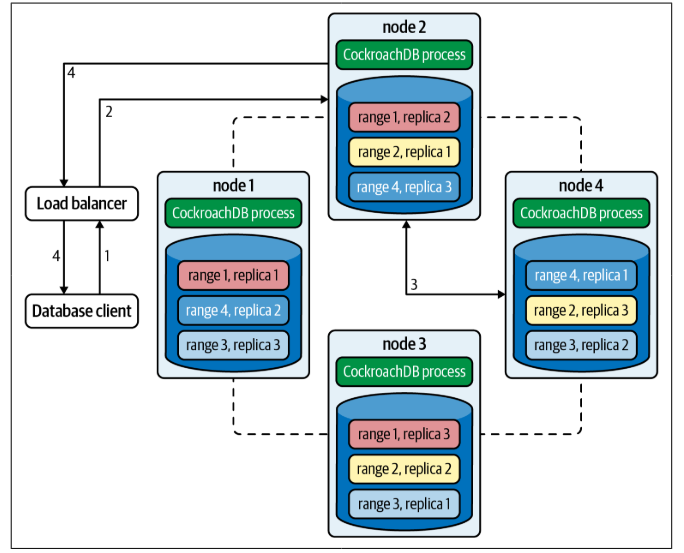
\includegraphics[width=0.5\linewidth]{images/CockroachdbArc.png}
    \caption{Kiến trúc một cụm trong CockroachDB \cite{CockroachDBGuide}}
    \label{fig:CockroachdbArc}
\end{figure}


Khi xét về cấu trúc cơ bản, một triển khai CockroachDB gồm nhiều quá trình máy chủ cơ sở dữ liệu. Mỗi máy chủ này được cấp phát lưu trữ độc lập, tuân theo mô hình cụm cơ sở dữ liệu shared-nothing. Điều này đồng nghĩa với việc mỗi node trong cụm CockroachDB hoạt động độc lập và không phụ thuộc vào node khác, không có sự phân biệt về vai trò giữa chính hay phụ. Lưu trữ này thường trực tiếp lưu trong máy chủ chạy dịch vụ CockroachDB, nhưng cũng có thể được cấu hình trên hệ thống lưu trữ chung. Dữ liệu được phân phối đều đặn qua cụm và có ít nhất ba bản sao được lưu trữ trên các máy chủ trong cụm.


Hình \ref{fig:layercrdb} minh họa cấu trúc các tầng của CockroachDB là một kiến trúc tầng phức tạp, mỗi tầng đóng một vai trò riêng biệt trong việc xử lý dữ liệu và yêu cầu.

\textbf{Tầng SQL}

Tầng SQL của CockroachDB là một thành phần cốt lõi, đóng vai trò cầu nối giữa người dùng và hệ thống cơ sở dữ liệu phân tán. Tầng này cho phép người dùng thực hiện các truy vấn và thao tác dữ liệu bằng ngôn ngữ SQL, một ngôn ngữ truy vấn chuẩn trong ngành được rất nhiều hệ quản trị cơ sở dữ liệu sử dụng.

Tầng SQL của CockroachDB tương thích cao với chuẩn SQL của PostgreSQL, điều này có nghĩa là nhiều ứng dụng được thiết kế cho PostgreSQL có thể chạy trên CockroachDB mà không cần chỉnh sửa lớn hoặc không chỉnh sửa. Sự tương thích này bao gồm hỗ trợ cho một loạt các tính năng SQL như truy vấn dữ liệu, các phép toán trên tập hợp, hàm tổng hợp, và giao dịch theo chuẩn ACID, cho phép người dùng thực hiện các truy vấn phức tạp và đa dạng.

Trong tầng SQL, truy vấn của người dùng được phân tích cú pháp và biên dịch thành một kế hoạch truy vấn. Quá trình này bao gồm việc xác định cách tốt nhất để thực hiện truy vấn dựa trên cấu trúc dữ liệu và các chỉ mục có sẵn. CockroachDB sử dụng một trình tối ưu hóa truy vấn mạnh mẽ để tạo ra kế hoạch hiệu quả nhất, giảm thiểu thời gian và tài nguyên cần thiết để trả về kết quả.


\textbf{Tầng Transaction}

Tầng Transaction đảm bảo tính toàn vẹn giao dịch theo nguyên tắc all or nothing, tức là tất cả các hoạt động trong một giao dịch phải hoàn thành hoàn toàn hoặc không được thực hiện. Cách tiếp cận này, với độ cô lập giao dịch mặc định là SERIALIZABLE—theo tiêu chuẩn ANSI SQL—đảm bảo rằng mỗi giao dịch diễn ra như thể nó được thực hiện trong một môi trường hoàn toàn độc lập.

\textbf{Tầng Distribution}

CockroachDB là một yếu tố quan trọng, giúp nền tảng này quản lý và phối hợp các hoạt động trên cụm dữ liệu phân tán. Đây là cách CockroachDB xử lý dữ liệu trên nhiều node một cách hiệu quả, bảo đảm tính sẵn sàng và nhất quán trong mọi giao dịch.

Đầu tiên, CockroachDB chia dữ các range, mỗi range có kích thước khoảng 128MB. Dữ liệu được phân tán tự động giữa các node trong cụm, nhằm mục đích cải thiện độ trễ và khả năng mở rộng. Mỗi range của dữ liệu không chỉ được lưu trữ tại một node mà còn được sao chép ra nhiều node khác, điều này đảm bảo độ bền và tính khả dụng cao của dữ liệu.

Để duy trì nhất quán dữ liệu trên toàn cụm, CockroachDB áp dụng giao thức Raft, đảm bảo rằng mọi thay đổi đối với dữ liệu đều được phản ánh một cách nhất quán trên tất cả các bản sao, giúp giảm thiểu lỗi và xung đột trong dữ liệu.

Bên cạnh việc sao chép, CockroachDB cũng sử dụng phân vùng dữ liệu để cải thiện hiệu suất truy vấn và cân bằng tải. Dữ liệu được phân bổ theo cách chiến lược trên các node để tối ưu hóa truy cập dữ liệu và quản lý tải truy cập hiệu quả, giảm độ trễ trong các truy vấn và tăng tốc độ xử lý.

Cuối cùng, CockroachDB có khả năng tự động cân bằng tải bằng cách liên tục điều chỉnh phân bổ dữ liệu giữa các node. Khi có sự thay đổi về tải truy cập hoặc dung lượng lưu trữ, hệ thống sẽ tự động chuyển dữ liệu giữa các node để duy trì hiệu quả hoạt động. Ngoài ra, trong trường hợp node gặp sự cố, CockroachDB có thể phục hồi nhanh chóng bằng cách tái tạo các bản sao range từ các node khác, giảm thiểu thời gian chết và bảo vệ dữ liệu.

\textbf{Tầng Replication}

Replication là một trong những thành phần chính giúp đảm bảo độ bền và tính khả dụng của dữ liệu trong một hệ thống phân tán. Tầng này quản lý việc sao chép dữ liệu giữa các node trong cụm, đảm bảo rằng dữ liệu luôn được bảo vệ và có thể truy cập ngay cả trong trường hợp sự cố.

Để quản lý và điều chỉnh việc phân bố ranges và sao chép, CockroachDB liên tục theo dõi và theo dõi tình trạng của các node. Hệ thống sử dụng thông tin này để tự động cân bằng lại dữ liệu giữa các node, tối ưu hóa hiệu suất và độ tin cậy. Khi một node mới được thêm vào cụm, CockroachDB có thể tự động sao chép và cân bằng ranges để tận dụng tài nguyên từ node mới, giảm bớt gánh nặng cho các node khác.

Khi một node bị lỗi, CockroachDB sẽ sử dụng các bản sao còn lại của dữ liệu để khôi phục lại range bị ảnh hưởng trên node khác. Quá trình này đảm bảo rằng cơ sở dữ liệu luôn khả dụng và dữ liệu không bị mất ngay cả khi xảy ra sự cố phần cứng.

\textbf{Tầng Storage}

Mỗi node trong CockroachDB chứa ít nhất một store, là đơn vị lưu trữ vật lý nơi dữ liệu được ghi và đọc từ đĩa. Mỗi store khởi tạo khi node bắt đầu hoạt động và chứa hai thành phần của Pebble engine: một dành cho dữ liệu tạm của các truy vấn SQL phân tán và một cho dữ liệu còn lại của node. Block cache được chia sẻ giữa tất cả các store trong node hỗ trợ cải thiện hiệu suất truy cập dữ liệu và phân phối thông minh dữ liệu giữa các stores, đảm bảo khả năng chịu lỗi và duy trì tính sẵn sàng cao của hệ thống.

Mỗi tầng trong kiến trúc CockroachDB được thiết kế để đáp ứng các yêu cầu kỹ thuật cụ thể, từ tối ưu hóa truy vấn đến đảm bảo độ tin cậy và sẵn sàng cao, đồng thời duy trì sự nhất quán và toàn vẹn dữ liệu trong môi trường phân tán.



\begin{figure}
    \centering
    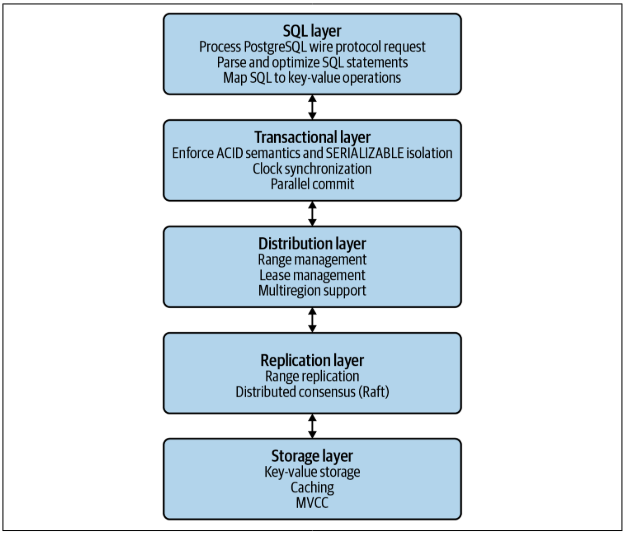
\includegraphics[width=0.8\linewidth]{images/layercrdb.png}
    \caption{Kiến trúc tầng trong CockroachDB \cite{CockroachDBGuide}}
    \label{fig:layercrdb}
\end{figure}


\subsection{TiDB}

TiDB là một hệ thống quản lý cơ sở dữ liệu phân tán được thiết kế để cung cấp khả năng tương thích cao với MySQL, đồng thời hỗ trợ các yêu cầu về khả năng chịu lỗi, độ tin cậy và mở rộng quy mô lớn. Kiến trúc của TiDB được thiết kế để tối ưu hóa cả hiệu suất giao dịch và truy vấn phân tích, làm cho nó trở thành một lựa chọn lý tưởng cho các doanh nghiệp cần một giải pháp cơ sở dữ liệu có khả năng phục vụ toàn cầu.

Kiến trúc TiDB gồm 3 thành phần chính là TiDB Server, Placement Driver server và Storage server như trinh hình \ref{fig:TiDBArchiteture}.


\begin{figure}
    \centering
    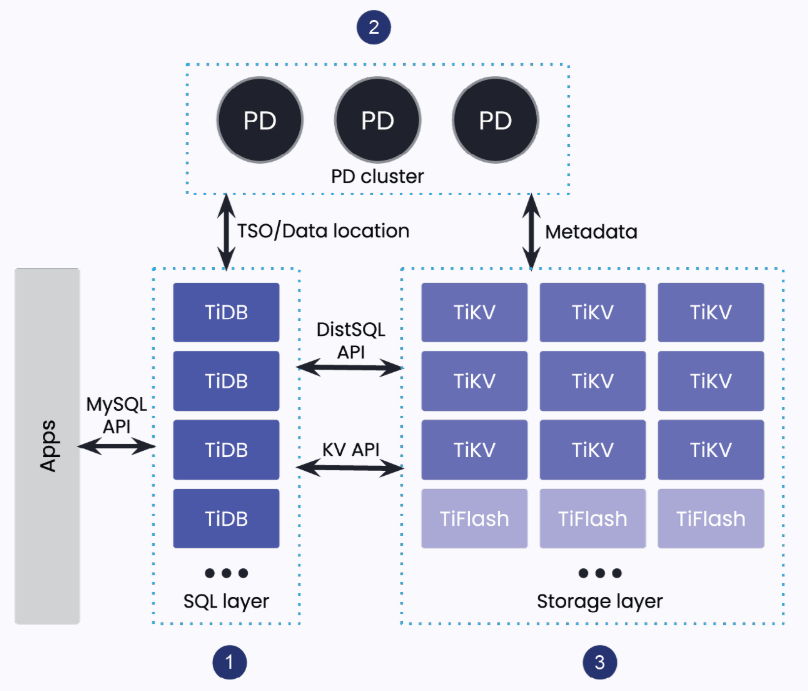
\includegraphics[width=0.6\linewidth]{images/TiDBArchiteture.png}
    \caption{Kiến trúc của TiDB\protect\footnotemark}
    \label{fig:TiDBArchiteture}
\end{figure}
\footnotetext{\url{https://static.pingcap.com/files/2024/02/01183648/TiDB_vs_MySQL_whitepaper.pdf}.}




\textbf{TiDB}

SQL Layer: Đây là lớp tiếp nhận các truy vấn SQL từ clients và chịu trách nhiệm phân tích cú pháp và tối ưu hóa các truy vấn. Lớp này hoạt động như một stateless server, có thể mở rộng ngang một cách dễ dàng bằng cách thêm các instances.

TiDB hỗ trợ giao thức MySQL, cho phép nó hoạt động và tích hợp một cách mượt mà với hầu hết các ứng dụng MySQL hiện có mà không cần chỉnh sửa.

\textbf{Placement Driver (PD) Layer}

Cluster Management: PD là thành phần quản lý tập trung của TiDB, chịu trách nhiệm cho việc lưu trữ metadata và quản lý và phân bổ dữ liệu giữa các TiKV nodes. PD cũng cân bằng tải và tối ưu hóa việc phân bổ dữ liệu trong cụm.

Scheduler: PD lên kế hoạch cho việc phân chia và sao chép dữ liệu, đảm bảo dữ liệu được sao chép và phân phối hợp lý giữa các nodes để cải thiện độ tin cậy và khả năng sẵn có.


\textbf{TiKV}

Storage Engine: TiKV là một engine lưu trữ phân tán, key-value, được xây dựng dựa trên thiết kế của Google Spanner. TiKV lưu trữ dữ liệu thực tế và xử lý các truy vấn dữ liệu cấp thấp từ TiDB layer.

Raft Consensus: TiKV sử dụng thuật toán đồng thuận Raft để đảm bảo tính nhất quán trong sao chép dữ liệu giữa các sao chép, từ đó nâng cao độ tin cậy của hệ thống.

Khả năng mở rộng theo chiều nganh: TiKV có thể mở rộng ngang một cách linh hoạt khi cần thêm tài nguyên, mà không gây ra gián đoạn.

\subsection{YugabyteDB}

\begin{figure}
    \centering
    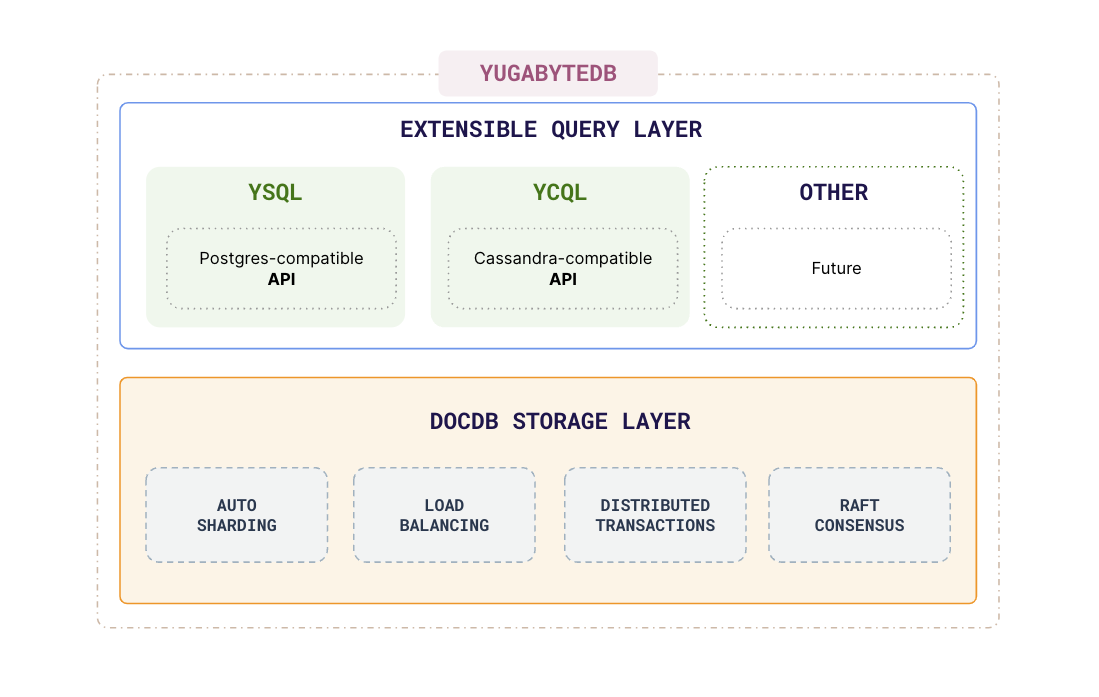
\includegraphics[width=0.6\linewidth]{images/YugaArchitecture.png}
    \caption{Kiến trúc của Yugabyte \protect\footnotemark}
    \label{fig:YugaArchitecture}
\end{figure}
\footnotetext{\url{https://docs.yugabyte.com/preview/architecture}.}



YugabyteDB là hệ thống quản lý cơ sở dữ liệu phân tán, mã nguồn mở, được thiết kế để đáp ứng nhu cầu về khả năng mở rộng cao và tính sẵn có liên tục cho các ứng dụng hiện đại. Với kiến trúc kết hợp linh hoạt giữa SQL và NoSQL, YugabyteDB mang lại sự đa dạng trong quản lý dữ liệu, tối ưu cho cả hai hình thức ứng dụng.

YugabyteDB bao gồm hai thành phần chính: YSQL và YCQL. YSQL là một lớp SQL hoàn chỉnh, tương thích với PostgreSQL, cho phép YugabyteDB hỗ trợ ứng dụng dựa trên SQL mà không cần chỉnh sửa. YCQL, ngược lại, là giao diện truy vấn dựa trên Apache Cassandra, được tối ưu hóa cho các hoạt động NoSQL với khả năng mở rộng cao và độ chịu lỗi tốt.

Sự đảm bảo về tính nhất quán của dữ liệu trên nhiều node trong cụm được hỗ trợ bởi thuật toán đồng thuận RAFT. Việc tổ chức dữ liệu thành các phân vùng, với mỗi phân vùng có thể có một hoặc nhiều bản sao, không chỉ củng cố độ tin cậy và khả năng chịu lỗi của hệ thống mà còn cải thiện hiệu suất đọc.

Hình \ref{fig:YugaArchitecture} mô tả kiến trúc của YugabyteDB được minh họa qua sự phân chia rõ ràng thành hai tầng cơ bản: tầng truy vấn và tầng lưu trữ. Tầng truy vấn, hoạt động như bộ não của hệ thống, chịu trách nhiệm xử lý yêu cầu của người dùng và điều hướng chúng tới vị trí dữ liệu thích hợp. Tầng này quan trọng trong việc giải mã và thực thi các lệnh SQL hoặc NoSQL tùy theo giao diện sử dụng: YSQL cho các tương tác giống SQL và YCQL cho các hoạt động NoSQL.

Tầng lưu trữ, đảm nhiệm việc quản lý vật lý dữ liệu, bảo đảm dữ liệu được lưu trữ một cách hiệu quả trên đĩa cứng. Tầng này quản lý các nhiệm vụ quan trọng như sao chép để bảo vệ dữ liệu khỏi mất mát và xử lý tính nhất quán để duy trì tính toàn vẹn của dữ liệu trên nhiều node. Ngoài ra, tầng lưu trữ sử dụng các thuật toán tiên tiến để tối ưu hóa quá trình truy xuất và lưu trữ dữ liệu, đảm bảo hiệu suất cao và độ bền trong các thao tác dữ liệu.

Các thành phần chính của YugabyteDB bao gồm:

Lớp Lưu Trữ (Storage Layer)
Tầng lưu trữ chịu trách nhiệm cho việc lưu giữ vật lý dữ liệu trên các thiết bị lưu trữ. Nó sử dụng DocDB, một hệ thống lưu trữ dạng key-value, được xây dựng dựa trên RocksDB, để quản lý hiệu quả việc lưu trữ và truy xuất dữ liệu. Thành phần này đảm bảo tính nhất quán và độ bền của dữ liệu thông qua cơ chế sao chép và phục hồi sau sự cố.

Sharding
Sharding trong YugabyteDB được thực hiện thông qua việc phân chia dữ liệu thành nhiều tablets, mỗi tablet là một khối dữ liệu độc lập được quản lý và phân bổ trên các node trong cụm. Điều này giúp cải thiện đáng kể khả năng mở rộng và hiệu suất truy xuất dữ liệu bằng cách phân tán tải và giảm thiểu điểm nghẽn.

Sao Chép (Replication)
Sao chép dữ liệu giữa các node được quản lý bởi thuật toán đồng thuận RAFT, đảm bảo tính nhất quán trong cụm. Mỗi tablet có một leader và nhiều followers, với leader chịu trách nhiệm xử lý các yêu cầu ghi và followers hỗ trợ đọc dữ liệu, từ đó cải thiện khả năng chịu lỗi và độ sẵn sàng của hệ thống.

Transactions
YugabyteDB hỗ trợ giao dịch đa bảng với đảm bảo tính toàn vẹn dữ liệu theo mô hình ACID. Cơ chế giao dịch này được xây dựng dựa trên cơ sở của snapshot isolation, cho phép các giao dịch song song diễn ra mà không ảnh hưởng lẫn nhau, đảm bảo hiệu suất và tính nhất quán cao.

Master Server
Master Server trong YugabyteDB chịu trách nhiệm quản lý toàn bộ metadata của cụm, bao gồm cấu hình cụm, schema của các bảng và trạng thái của các tablets. Nó cũng phụ trách việc cân bằng tải và phân bổ tài nguyên giữa các node, giúp tối ưu hóa hiệu suất và khả năng phục hồi.

TServer (Tablet Server)
TServer là nơi xử lý trực tiếp các yêu cầu đọc và ghi dữ liệu trên các tablets mà nó quản lý. Mỗi TServer chịu trách nhiệm cho một nhóm các tablets, thực hiện các thao tác dữ liệu và phối hợp với các TServer khác cùng với Master Server để đảm bảo hoạt động ổn định và hiệu quả của hệ thống.

Các thành phần này, khi làm việc cùng nhau, tạo nên một hệ thống cơ sở dữ liệu mạnh mẽ, linh hoạt, và đáng tin cậy, đáp ứng nhu cầu của các ứng dụng quan trọng trong thời đại số hiện nay.

Với những cải tiến này, YugabyteDB đem lại một giải pháp cơ sở dữ liệu mạnh mẽ, đáp ứng nhu cầu về hiệu suất cao, khả năng mở rộng và tính sẵn sàng cao cho các ứng dụng quan trọng trong thời đại số.

\subsection{Greenplum}


Greenplum là một hệ thống quản lý cơ sở dữ liệu phân tán, được thiết kế đặc biệt để xử lý và phân tích dữ liệu lớn (big data). Phát triển dựa trên nền tảng PostgreSQL, hệ thống này tận dụng khả năng mở rộng và tính năng xử lý song song, cung cấp một giải pháp mạnh mẽ và linh hoạt cho các doanh nghiệp cần xử lý khối lượng dữ liệu khổng lồ.

Một trong những điểm nổi bật của Greenplum là khả năng mở rộng ngang. Điều này cho phép hệ thống tăng thêm năng lực xử lý và lưu trữ mà không cần đầu tư lớn vào cơ sở hạ tầng. Với kiến trúc phân tán, Greenplum có thể dễ dàng thêm các node mới mà không gây gián đoạn hoạt động. Điều này đảm bảo khả năng phản ứng nhanh chóng với sự tăng trưởng đột ngột của dữ liệu, giúp các tổ chức duy trì hoạt động ổn định và hiệu quả.

Greenplum được xây dựng dựa trên kiến trúc xử lý song song đại trà (Massively Parallel Processing - MPP). Kiến trúc này cho phép nhiều bộ vi xử lý thực hiện tác vụ độc lập nhưng đồng thời, giúp xử lý hiệu quả các dữ liệu lớn và phức tạp. Điều này được thực hiện qua các segment độc lập, mỗi segment xử lý một phần dữ liệu, từ đó cắt giảm độ trễ và tối đa hóa hiệu suất khi thực hiện các truy vấn phức tạp.

Greenplum được tối ưu hóa để hỗ trợ cả xử lý giao dịch trực tuyến (Online Transaction Processing - OLTP) và xử lý phân tích trực tuyến (Online Analytical Processing - OLAP) trên cùng một hệ thống. Sự tích hợp này giúp giảm thiểu sự phức tạp trong cơ sở dữ liệu và tiết kiệm chi phí bằng cách loại bỏ nhu cầu duy trì nhiều hệ thống riêng biệt. Greenplum sử dụng giao thức cam kết một pha (One-Phase Commit Protocol) cho các giao dịch chỉ liên quan đến một segment duy nhất, giúp cải thiện hiệu suất và giảm thời gian đáp ứng cho các truy vấn OLTP.

Ngoài các truy vấn SQL cơ bản, Greenplum còn cung cấp các công cụ phân tích dữ liệu nâng cao như học máy và xử lý dữ liệu lớn. Những công cụ này giúp đơn giản hóa và hiệu quả hóa việc phân tích dữ liệu phức tạp, giúp tổ chức trích xuất giá trị tối đa từ dữ liệu lớn. Điều này đặc biệt quan trọng trong bối cảnh các doanh nghiệp ngày càng phải đối mặt với khối lượng dữ liệu ngày một tăng và yêu cầu phân tích ngày càng phức tạp.

Tổng hợp lại, Greenplum là một giải pháp quản lý dữ liệu đa năng, hiệu quả và linh hoạt, phù hợp cho cả hoạt động xử lý giao dịch hàng ngày và các tác vụ phân tích dữ liệu sâu rộng. Khả năng mở rộng ngang của hệ thống cho phép dễ dàng thêm các node mới vào cụm mà không gây gián đoạn dịch vụ hiện hữu. Điều này đặc biệt quan trọng khi cần xử lý khối lượng dữ liệu tăng lên một cách nhanh chóng và hiệu quả, giúp các tổ chức duy trì tính cạnh tranh và đáp ứng nhu cầu phát triển không ngừng của thị trường.

\subsubsection{Kiến trúc của Greenplum}

Greenplum với mỗi node có hiệu suất tương đương cơ sở dữ liệu MPP kiến trúc của hệ thống. Hình \ref{fig:gp-architecture} mô tả kiến trúc của Greenplum.

\begin{figure}[htbp]
\centerline{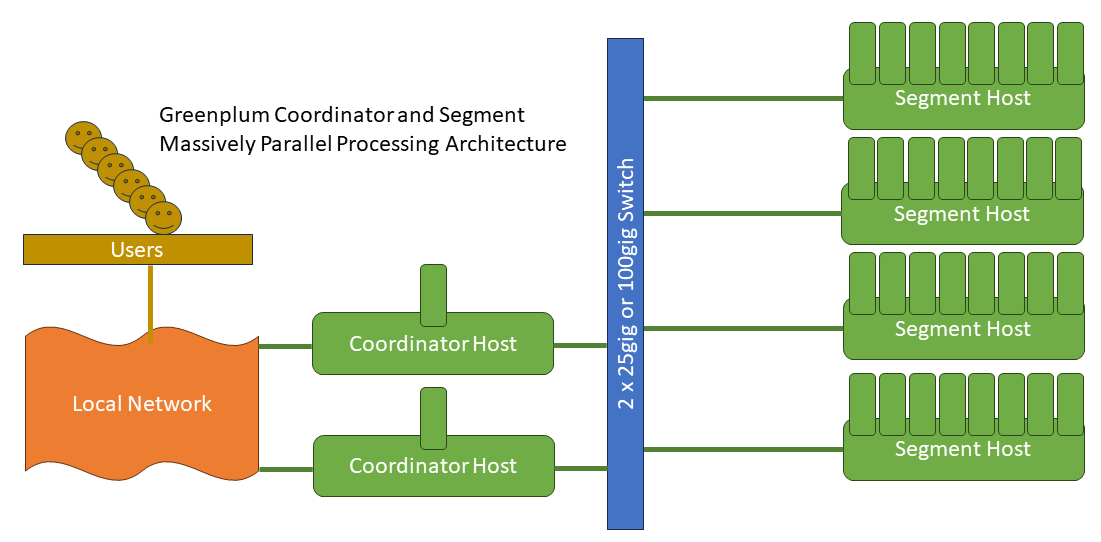
\includegraphics[scale=.4]{images/gp-architecture.png}}
\captionsetup{font=Large}
\caption{Kiến trúc hệ thống cơ sở dữ liệu Greenplum\protect\footnotemark.  }
\label{fig:gp-architecture}
\end{figure}
\footnotetext{\url{https://docs.vmware.com/en/VMware-Greenplum/7/greenplum-database/admin_guide-intro-arch_overview.html}.}


Greenplum là hệ thống cơ sở dữ liệu được xây dựng dựa trên kiến
trúc MPP, được tối ưu hóa để xử lý dữ liệu lớn và phân tích.


\paragraph{Coordinator}

Coordinator trong kiến trúc Greenplum là nơi quản lý và điều phối
toàn bộ hoạt động của cơ sở dữ liệu. Hình \ref{fig:admin_guide-graphics-standby_coordinator} Mô tả coordinator trong kiến trúc Greenplum.
Dưới đây là các yếu tố cụ thể:


\begin{figure}[htbp]
\centerline{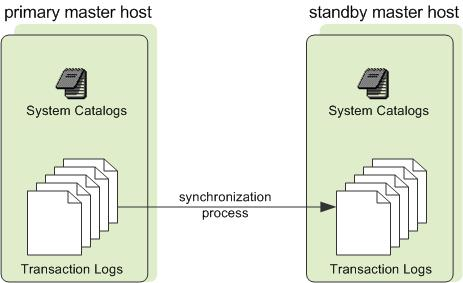
\includegraphics[scale=.7]{images/admin_guide-graphics-standby_coordinator.jpg}}
\captionsetup{font=Large}
\caption{Coordinator trong kiến trúc Greenplum \protect\footnotemark}
\label{fig:admin_guide-graphics-standby_coordinator}
\end{figure}
\footnotetext{\url{https://docs.vmware.com/en/VMware-Greenplum/7/greenplum-database/admin_guide-intro-arch_overview.html}.}

Quản lý truy vấn và điều phối: Coordinator nhận các truy vấn từ ứng dụng người dùng và chịu trách nhiệm phân tích cú pháp, tối ưu hóa truy vấn, và lập kế hoạch thực thi truy vấn. Nó phân phối các phần của truy vấn đã được tối ưu hóa đến các segment nodes để thực hiện.


Duy trì Metadata: Coordinator duy trì danh mục (catalog) của cơ sở dữ liệu, nơi lưu giữ thông tin về sơ đồ, dữ liệu, và cấu trúc của các bảng, cũng như các thông tin thống kê cần thiết cho việc tối ưu hóa truy vấn.

Quản lý giao dịch: Coordinator xử lý và quản lý các giao dịch, đảm bảo tính toàn vẹn, nhất quán, và cô lập dữ liệu. Nó sử dụng giao thức cam kết hai pha (two-phase commit protocol) để đảm bảo các thay đổi được thực hiện một cách đồng nhất trên tất cả các segment nodes.


Quản lý Tài nguyên: Coordinator quản lý các nguồn tài nguyên như bộ nhớ và CPU cho các truy vấn và có thể thiết lập các ưu tiên dựa trên chính sách quản lý tài nguyên.

Phục hồi và Sao lưu: Trong trường hợp có sự cố, master host có trách nhiệm khởi tạo các quy trình sao lưu và phục hồi để bảo đảm tính sẵn sàng và liên tục của hệ thống.

Monitoring và Logging: Coordinator cũng có trách nhiệm giám sát hoạt động của cả hệ thống và ghi lại các sự kiện hệ thống, giúp trong việc phân tích hiệu suất và khắc phục sự cố. Coordinator đóng vai trò trung tâm trong kiến trúc Greenplum, đảm nhiệm nhiều chức năng quan trọng từ việc quản lý truy vấn đến quản lý tài nguyên và đảm bảo tính ổn định của hệ thống.

\paragraph{Segment}

Trong kiến trúc Greenplum, segment là những máy chủ cơ sở dữ liệu hoặc
nodes làm việc song song để xử lý và lưu trữ dữ liệu. Dưới đây là mô tả chi tiết về segment trong Greenplum:

Xử lý dữ liệu song song: Mỗi segment là một node xử lý độc lập, chạy một instance của cơ sở dữ liệu PostgreSQL. Các segment làm việc cùng nhau một cách song song, mỗi segment xử lý một phần của truy vấn tổng thể và dữ liệu liên quan.

Lưu trữ phân tán: Dữ liệu trong Greenplum được phân phối đều ra các segment. Mỗi segment chứa một phần dữ liệu và được quản lý độc lập.
Kỹ thuật phân phối có thể bao gồm hash-based, random, hoặc các phân vùng
dữ liệu cụ thể. 

Tính độc lập và kiến trúc shared-nothing:
Mỗi segment có bộ nhớ và không gian lưu trữ của riêng mình, tuân theo kiến trúc shared-nothing. Điều này đảm bảo rằng không có sự phụ thuộc giữa các segment, giảm thiểu các điểm nghẽn và cải thiện hiệu suất.

Tự động phục hồi: Greenplum có khả năng tự động phục hồi từ lỗi ở cấp segment. Khi một segment gặp sự cố, Greenplum có thể chuyển công việc sang một segment dự bị hoặc phục hồi segment bị lỗi.

Hiệu suất cao và khả năng mở rộng: Do mỗi segment xử lý một phần nhỏ của dữ liệu, hệ thống có thể mở rộng quy mô một cách linh hoạt bằng cách thêm segment vào hệ thống để xử lý khối lượng dữ liệu lớn hơn.
Sự mở rộng này có thể được thực hiện mà không cần thay đổi cấu trúc hoặc
cấu hình của các segment hiện có.

Quản lý và giám sát:
Mỗi segment được giám sát bởi coordinator, đảm bảo rằng nó hoạt động đúng
và hiệu quả. Coordinator có thể giám sát tình trạng và hiệu suất của từng segment, và thực hiện các điều chỉnh khi cần thiết.

Cân bằng tải: Greenplum sử dụng cơ chế cân bằng tải để đảm bảo rằng không có segment nào bị quá tải hoặc nhàn rỗi.
Việc phân phối công việc giữa các segment được thực hiện dựa trên cấu hình và tình trạng hiện tại của hệ thống.

Segments đóng vai trò quan trọng trong việc đảm bảo khả năng xử lý dữ liệu lớn và phức tạp của Greenplum, giúp nó trở thành một giải pháp mạnh mẽ cho việc kho dữ liệu và phân tích dữ liệu quy mô lớn.

\paragraph{Node Motion}

Greenplum đã giới thiệu một node kế hoạch mới có tên là Motion để thực hiện việc di chuyển dữ liệu này. Node Motion sử dụng mạng để gửi và nhận dữ liệu từ các segment khác nhau, tạo điều kiện cho việc phân chia kế hoạch truy vấn thành nhiều phần khác nhau, mỗi phần được gọi là một slice. Mỗi slice sau đó được thực thi bởi một nhóm các quá trình phân tán, được gọi chung là gang. Với việc sử dụng node Motion và khái niệm gang, kế hoạch truy vấn và quá trình thực thi của Greenplum trở nên phân tán. Kế hoạch sẽ được gửi đến từng quá trình, và mỗi quá trình sẽ thực thi phần slice của kế hoạch dựa trên ngữ cảnh và trạng thái cục bộ của mình. Điều này phản ánh kỹ thuật Single Program Multiple Data (SPMD), nơi cùng một kế hoạch được phân phát đến các nhóm quá trình trên khắp cụm. Các quá trình khác nhau được tạo ra bởi các segment khác nhau sẽ có ngữ cảnh, trạng thái và dữ liệu cục bộ riêng của chúng. Hình \ref{fig:plan} ví dụ về kế hoạch phân tán và thực thi của Greenplum.

\begin{figure}[htbp]
\centerline{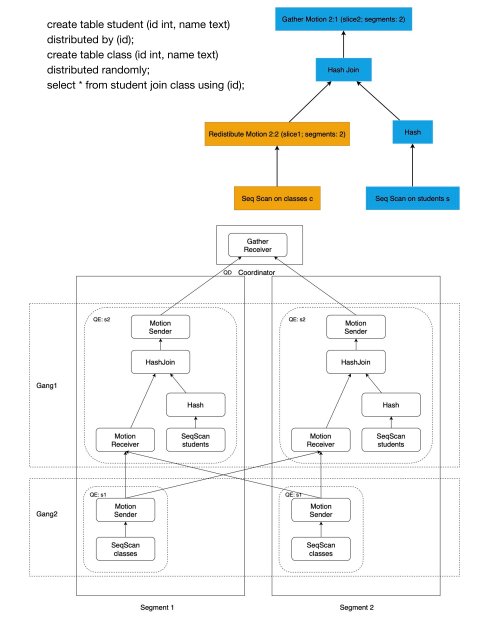
\includegraphics[scale=.8]{images/plan.PNG}}
\captionsetup{font=Large}
\caption{Kế hoạch phân tán và thực thi của Greenplum \cite{lyu2021greenplum}}
\label{fig:plan}
\end{figure}

Từ hình \ref{fig:plan} cho thấy Greenplum bảng student được tạo với việc phân phối dữ liệu dựa trên cột id. Điều này có nghĩa là dữ liệu sẽ được phân chia giữa các segment sao cho mỗi id student sẽ chỉ tồn tại trên một segment cụ thể. Bảng class được tạo với dữ liệu phân phối một cách ngẫu nhiên, không theo một quy tắc cụ thể nào. Khi truy vấn SELECT * FROM student JOIN class USING (id); được thực hiện, hệ thống sẽ tạo ra một kế hoạch thực thi phân tán. Kế hoạch này xác định làm thế nào dữ liệu từ cả hai bảng sẽ được kết hợp dựa trên cột id. Các segment thực hiện quét tuần tự (Seq Scan) trên bảng student và class để lấy các bản ghi cần thiết cho việc thực hiện join. Motion Sender: Nằm trên mỗi Motion Sender: Nằm trên mỗi segment, sẽ xác định các bản ghi từ bảng
class mà cần được di chuyển để join với bảng student.
Motion Receiver nằm trên segment đích, sẽ nhận các bản ghi từ bảng class
đã được gửi qua và chuẩn bị cho việc join, sẽ xác định các bản ghi từ bảng class mà cần được di chuyển để join với bảng student. Motion Receiver nằm trên segment đích, sẽ nhận các bản ghi từ bảng class đã được gửi qua và chuẩn bị cho việc join. Trong mỗi segment, một Hash Join được thực hiện giữa các bản ghi từ bảng student và các bản ghi từ bảng class đã được di chuyển đến. Đây là bước dữ liệu từ bảng class có thể cần được phân phối lại (redistributed) giữa các phân đoạn để đảm bảo rằng mỗi student có thể được join với đúngclass dựa trên id. Sau khi join được thực hiện trên các phân đoạn, kết quả sau cùng sẽ được gửi về cho Gather Receiver ở coordinator, nơi tất cả kết quả từ các phân đoạn được tổng hợp lại. Coordinator sau đó sẽ trả về kết quả cuối cùng của truy vấn join cho người dùng hoặc ứng dụng đã yêu cầu truy vấn. Trong quá trình này, Gang1 và Gang2 có thể hiểu là nhóm các quá trình làm việc trên các phân đoạn khác nhau để thực hiện các phần khác nhau của kế hoạch thực thi (ví dụ: quét tuần tự, join). Mỗi gang có thể gồm nhiều slice, tương ứng với một phần của công việc cần thực hiện trên mỗi phân
đoạn.

\paragraph{Khóa}

Trong Greenplum, khóa được sử dụng rộng rãi để ngăn chặn các tình huống
đua tranh ở nhiều cấp độ khác nhau. Có ba loại khóa khác nhau được thiết kế cho các trường hợp sử dụng khác nhau: khóa quay vòng (spin locks), khóa nhẹ (LWlocks), và khóa đối tượng (Object locks).

Khóa quay vòng là loại khóa cực kỳ đơn giản, thường được sử dụng để bảo
vệ các cấu trúc dữ liệu nhỏ và đơn giản. Khi một tiến trình cần truy cập vào một tài nguyên được bảo vệ bởi một spin lock, nó sẽ liên tục kiểm tra (hay quay vòng) để xem khóa có sẵn hay không. Nếu khóa không sẵn có, tiến trình sẽ tiếp tục vòng lặp này cho đến khi nó có thể giành được khóa. Spin locks phù hợp khi thời gian giữ khóa ngắn, vì nó yêu cầu tiến trình tiêu tốn CPU cho việc quay vòng kiểm tra khóa. Nếu một tiến trình giữ spin lock trong thời gian dài, nó có thể gây ra hiệu suất kém vì các tiến trình khác sẽ phải chờ đợi trong vòng lặp quay vòng.
LWlocks phức tạp hơn spin locks và thường được sử dụng để bảo vệ các cấu
trúc dữ liệu lớn hơn hoặc các hoạt động phức tạp hơn. Chúng cho phép một
số mức độ đọc hoặc viết song song, và cung cấp một cơ chế chờ đợi hiệu quả
hơn so với việc quay vòng liên tục. Khi một tiến trình cần một LWlock nhưng không thể lấy được ngay lập tức, nó sẽ đi vào trạng thái chờ đợi thay vì quay vòng. Điều này giúp giảm tải cho CPU và cho phép xử lý các tiến trình khác trong khi đang chờ.

Khóa đối tượng: Là một cơ chế khóa ở cấp độ cao, được sử dụng để quản lý
truy cập và cập nhật trên các đối tượng cơ sở dữ liệu như bảng, bản ghi, và giao dịch. Đảm bảo rằng nhiều quá trình có thể đồng thời làm việc trên cùng một cơ sở dữ liệu mà không làm ảnh hưởng đến tính toàn vẹn và nhất quán của dữ liệu. Truy cập song song: Khi nhiều quá trình cần truy cập hoặc thao tác trên cùng một đối tượng, khóa đối tượng sẽ quản lý cách thức và mức độ mà mỗi quá trình có thể tương tác với đối tượng đó.

Bảng \ref{tab:khoadoituong} mô tả các cấp độ khóa trong khóa đối tượng: 

\begin{longtable}{|>{\raggedright\arraybackslash}p{6cm}|>{\raggedright\arraybackslash}p{1cm}|>{\raggedright\arraybackslash}p{2cm}|>{\raggedright\arraybackslash}p{2cm}|>{\raggedright\arraybackslash}p{5cm}|}
\hline
\textbf{Tên khóa} & \textbf{Mức độ} & \textbf{Xung đột} & \textbf{Lệnh} &\textbf{Mô tả}\\ 
\hline
AccessShareLock & 1 & 8 & select & Đây là chế độ khóa nhẹ nhất, thường được sử dụng cho các lệnh đọc dữ liệu không thay đổi dữ liệu (như SELECT). Nó chỉ xung đột với chế độ khóa cao nhất, AccessExclusiveLock, giúp cho nhiều quá trình có thể đọc cùng một dữ liệu cùng lúc. \\
\hline
RowShareLock  & 2 & 7, 8 & Select for update & Khóa này được áp dụng trong các thao tác SELECT FOR UPDATE. Nó khóa các hàng được chọn để cập nhật nhưng vẫn cho phép các giao dịch khác đọc các hàng này. \\
\hline
RowExclusiveLock & 3 & 5, 6, 7, 8 & Insert & Thường được sử dụng trong các thao tác INSERT. Nó ngăn các giao dịch khác sửa đổi cùng một hàng, nhằm đảm bảo tính toàn vẹn dữ liệu khi chèn. \\
\hline
ShareUpdateExclusiveLock & 4 & 4, 5, 6, 7, 8 & Vacuum (not full) & Thường được sử dụng trong các thao tác bảo trì như VACUUM (không phải toàn bộ). Khóa này hạn chế hơn để tránh xung đột trong các tác vụ bảo trì. \\
\hline
ShareLock & 5& 3, 4, 6, 7, 8 & Create index & Được áp dụng trong các thao tác như CREATE INDEX. Nó hạn chế hơn để bảo vệ cấu trúc của bảng trong khi chỉ mục đang được tạo. \\
\hline
ShareRowExclusiveLock & 6 & 3, 4, 5, 6, 7, 8 & Collation create & Được sử dụng trong các thao tác sửa đổi lược đồ, như tạo collation. Khóa này khá hạn chế để đảm bảo sự nhất quán của các thay đổi lược đồ. \\
\hline
ExclusiveLock & 7 & 2, 3, 4, 5, 6, 7, 8 & Concurrent refresh matview & Áp dụng trong các thao tác như REFRESH MATERIALIZED VIEW CONCURRENTLY. Nó rất hạn chế để ngăn các giao dịch khác thực hiện các thay đổi có thể xung đột với việc làm mới view. \\
\hline
AccessExclusiveLock & 8& 1, 2, 3, 4, 5, 6, 7, 8 & Alter table & Khóa hạn chế nhất, được sử dụng trong các thao tác như ALTER TABLE. Cơ bản nó khóa tất cả các thao tác khác trên bảng để đảm bảo tính toàn vẹn của các thay đổi cấu trúc lớn. \\
\hline
\caption{Mô tả các cấp độ khóa trong khóa đối tượng \cite{lyu2021greenplum}}
\label{tab:khoadoituong}
\end{longtable}



Khóa đối tượng phân biệt giữa các thao tác đọc và ghi, cho phép độc lập trong truy cập đọc trong khi quản lý cẩn thận truy cập bản ghi để tránh xung đột dữ liệu.

Trong môi trường hệ thống phân tán, việc xử lý và phát hiện deadlock trở thành một thách thức quan trọng do sự phức tạp của các quan hệ phụ thuộc giữa các tài nguyên và các quá trình. Deadlock có thể làm giảm hiệu quả của hệ thống và dẫn đến hậu quả nghiêm trọng về hiệu suất và độ tin cậy.



Trong môi trường cơ sở dữ liệu phân tán như Greenplum, việc phát hiện và giải quyết deadlock là cực kỳ quan trọng để đảm bảo hoạt động liền mạch và hiệu quả của hệ thống. Deadlock xảy ra khi có một hoặc nhiều tiến trình đang lẫn nhau chờ đợi nguồn lực được giải phóng bởi nhau, tạo thành một vòng lặp khóa không thể tự giải quyết. Thuật toán phát hiện deadlock toàn cầu như hình \ref{fig:algorithmGreenplum}  được thiết kế để xác định mối quan hệ chờ đợi này thông qua một đồ thị chờ đợi toàn cầu và tiến hành giải quyết các tình trạng bế tắc này.

Đồ thị này là một Đồ thị có hướng, trong đó mỗi node biểu diễn một tiến trình và mỗi cạnh hướng từ tiến trình này sang tiến trình khác cho biết tiến trình nguồn đang chờ đợi một tài nguyên từ tiến trình đích. Đồ thị này cung cấp một cái nhìn toàn diện về các mối quan hệ phụ thuộc giữa các tiến trình trong toàn bộ hệ thống.

Mỗi vòng lặp của thuật toán sẽ loại bỏ các đỉnh không có cạnh đi ra, tức là các tiến trình không chờ đợi bất kỳ tài nguyên nào từ tiến trình khác. Bước này giúp đơn giản hóa đồ thị và loại bỏ những tiến trình không liên quan đến tình trạng deadlock.

Sau khi loại bỏ các đỉnh không cần thiết, thuật toán tiếp tục xóa các cạnh trong phần đồ thị chờ đợi cục bộ. Điều này giúp làm giảm số lượng các mối quan hệ phụ thuộc và làm nổi bật những tiến trình còn lại có khả năng gây ra deadlock.

Nếu sau một vòng lặp không có đỉnh hoặc cạnh nào được loại bỏ, thuật toán sẽ kết thúc, vì không còn tiến trình nào bị chặn. Tuy nhiên, nếu vẫn tồn tại các cạnh trong đồ thị, điều này chỉ ra sự tồn tại của ít nhất một vòng lặp phụ thuộc, hay còn gọi là deadlock.



\begin{figure}
    \centering
    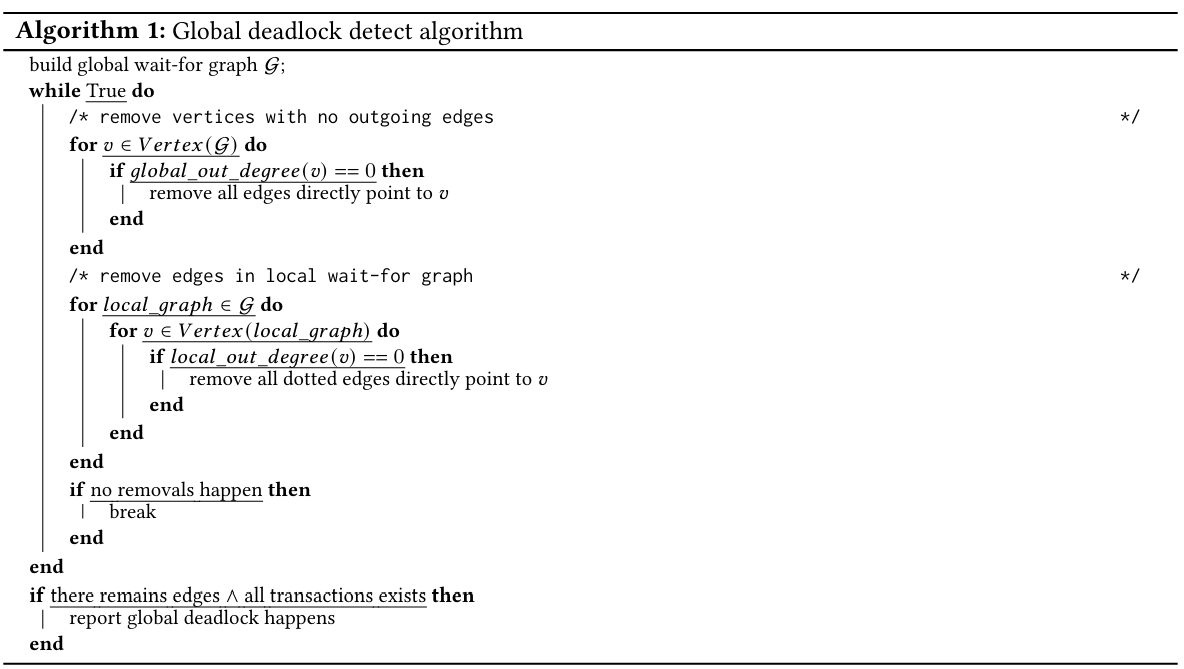
\includegraphics[width=0.8\linewidth]{images/algorithmGreenplum.png}
    \caption{Thuật toán global deadlock detect \cite{lyu2021greenplum}}
    \label{fig:algorithmGreenplum}
\end{figure}

Giả sử trong một hệ thống cơ sở dữ liệu phân tán, các tiến trình A, B và C lần lượt đang chờ đợi các tài nguyên X, Y và Z. Quá trình này được biểu diễn bởi đồ thị chờ đợi toàn cầu. Khi tiến hành loại bỏ các đỉnh và cạnh, nếu phát hiện các tiến trình còn lại vẫn có mối quan hệ chờ đợi không thể giải quyết nhận định có deadlock.

Greenplum áp dụng một loạt các chiến lược để phát hiện, giải quyết và phòng ngừa deadlock, đảm bảo tính ổn định và hiệu suất của hệ thống.

Khi phát hiện deadlock, Greenplum đầu tiên sẽ xác định node để giải quyết tình trạng bế tắc. Node được chọn dựa trên một số tiêu chí như:Chi phí xử lý ưu tiên hủy những tiến trình có chi phí hoàn tác thấp nhất. Độ ưu tiên của tiến trình có độ ưu tiên thấp hơn có thể được chọn làm node xử lý. Thời gian hoạt động trong một số trường hợp, tiến trình đã hoạt động trong khoảng thời gian ngắn có thể được chọn để giảm thiểu tác động.

Tiến trình được chọn sẽ bị hủy, và tất cả tài nguyên đang giữ sẽ được giải phóng. Greenplum cũng sẽ ghi nhận trạng thái của tiến trình vào thời điểm hủy để giúp phục hồi dữ liệu nếu cần.

Sau khi hủy bỏ tiến trình, Greenplum có thể tự động khởi động lại tiến trình nếu cần thiết, đảm bảo rằng công việc không bị gián đoạn. Việc khởi động lại phải đảm bảo không tái tạo lại các điều kiện dẫn đến deadlock.

Để giảm thiểu nguy cơ phát sinh deadlock, Greenplum áp dụng một số biện pháp phòng ngừa:

Khóa Hai Giai Đoạn (Two-Phase Locking): Đảm bảo rằng mọi khoá phải được giữ cho đến khi giao dịch hoàn tất, ngăn ngừa các khoá được giải phóng sớm gây ra bế tắc.

Ưu Tiên FIFO (First-In, First-Out): Điều này đảm bảo rằng các yêu cầu tài nguyên được xử lý theo thứ tự chúng được thực hiện, giảm thiểu khả năng xung đột.

Giám Sát Thời Gian Chờ Đợi: Theo dõi thời gian chờ đợi của các tiến trình để phát hiện sớm các tình huống có thể dẫn đến deadlock.




\section{Giải pháp đề xuất}

Trong thời đại kỹ thuật số hiện nay, việc quản lý và xử lý hiệu quả lượng dữ liệu ngày càng tăng trong các hệ thống thông tin là cực kỳ quan trọng. Các hệ thống cơ sở dữ liệu truyền thống như MSSQL đã chứng minh được nhiều giá trị, nhưng cũng bộc lộ những hạn chế nghiêm trọng trong việc đáp ứng nhu cầu về hiệu suất cao và khả năng mở rộng trong quản lý dữ liệu lớn. Như đã phân tích trong chương 1, các vấn đề như tốc độ truy vấn chậm, quản lý tài nguyên không hiệu quả, và hạn chế về khả năng mở đã làm suy giảm hiệu suất của các hệ thống quản lý thành viên trực tuyến như ASP.NET Membership database. Để giải quyết những vấn đề này sẽ đề xuất việc chuyển đổi cơ sở dữ liệu ASP.NET Membership từ MSSQL sang một hệ thống cơ sở dữ liệu phân tán.

\subsection{Chuyển đổi MSSQL sang cơ sở dữ liệu phân tán}

Việc chuyển đổi cơ sở dữ liệu ASP.NET Membership từ một hệ thống cơ sở dữ liệu tập trung như MSSQL sang một hệ thống cơ sở dữ liệu phân tán đòi hỏi phải thực hiện một loạt các bước kỹ thuật chi tiết. Quá trình này không chỉ bao gồm việc di chuyển dữ liệu mà còn phải đảm bảo rằng tất cả các chức năng và hiệu suất của hệ thống được duy trì hoặc cải thiện. Dưới đây là các bước chi tiết để thiết lập hệ thống cơ sở dữ liệu phân tán phù hợp cho ASP.NET Membership Database.

\subsubsection{Thiết lập hệ thống distributed database}

Để thiết lập một hệ thống cơ sở dữ liệu phân tán, bước đầu tiên là chuẩn bị môi trường phần cứng và phần mềm cần thiết. Mỗi node trong hệ thống cần có CPU đa nhân, RAM lớn và ổ đĩa SSD để đảm bảo hiệu suất cao. Hệ điều hành Linux, như CentOS hoặc Ubuntu, thường được sử dụng do tính ổn định và hiệu quả trong môi trường node. Các gói phần mềm cơ bản như SSH, rsync và các công cụ quản lý hệ thống khác cần được cài đặt trên mỗi node. Đối với mỗi hệ thống cụ thể, như Greenplum, CockroachDB, YugabyteDB và TiDB, có thể yêu cầu thêm các gói phần mềm và công cụ quản lý đặc thù.

Mạng nội bộ kết nối các node phải có tốc độ cao và ổn định để đảm bảo việc truyền tải dữ liệu nhanh chóng và giảm thiểu độ trễ. Các node cần có khả năng giao tiếp với nhau thông qua SSH không cần mật khẩu, điều này yêu cầu thiết lập các khóa SSH để xác thực không cần mật khẩu giữa các node. Điều này đảm bảo rằng các node có thể được quản lý từ xa một cách hiệu quả, tạo điều kiện cho việc cấu hình và triển khai hệ thống một cách dễ dàng và an toàn.

Việc lựa chọn phần mềm cơ sở dữ liệu phù hợp là rất quan trọng. Greenplum, CockroachDB, YugabyteDB và TiDB đều có những đặc điểm riêng biệt và ưu điểm cụ thể. Greenplum được thiết kế cho các tác vụ phân tích dữ liệu lớn nhờ kiến trúc MPP. CockroachDB và YugabyteDB nổi bật với tính nhất quán và khả năng chịu lỗi cao, trong khi TiDB cung cấp tính linh hoạt và khả năng tương thích cao với MySQL.

Quá trình cài đặt phần mềm bao gồm tải xuống và triển khai trên tất cả các node. Ví dụ, với Greenplum, cần thiết lập Master và Segment nodes. CockroachDB và YugabyteDB yêu cầu cài đặt và cấu hình các Replica nodes để đảm bảo tính sẵn sàng và độ chịu lỗi. TiDB đòi hỏi cài đặt các thành phần TiDB server, TiKV (key-value storage), và PD (Placement Driver) trên các node tương ứng. Đảm bảo rằng tất cả các node đều cài đặt cùng một phiên bản phần mềm để tránh xung đột trong quá trình vận hành.

Sau khi cài đặt, các tệp cấu hình của hệ thống cần được thiết lập để các node có thể hoạt động như một cụm đồng nhất. Đối với Greenplum, các tệp như pg\_hba.conf và postgresql.conf cần được cấu hình cẩn thận. CockroachDB sử dụng tệp cockroach.yaml để cấu hình các tham số hệ thống, YugabyteDB yêu cầu cấu hình trong yugabyted.conf, và TiDB sử dụng tidb.toml cùng với các cấu hình liên quan cho TiKV và PD. Các tệp cấu hình này xác định cách thức các node giao tiếp với nhau, cách dữ liệu được phân phối và các thông số khác liên quan đến hiệu suất và bảo mật.

Trong hệ thống Greenplum, các node được chia thành Master và Segment nodes, nơi Master node quản lý và điều phối các hoạt động. CockroachDB và YugabyteDB sử dụng mô hình phân tán ngang với các Replica nodes để đảm bảo tính sẵn sàng và độ chịu lỗi. TiDB cấu trúc thành các node TiDB server, TiKV và PD để phân chia nhiệm vụ quản lý và lưu trữ dữ liệu. Việc thiết lập các vai trò này giúp tối ưu hóa việc phân phối và quản lý dữ liệu trong hệ thống, đảm bảo rằng hệ thống có thể hoạt động một cách hiệu quả và ổn định.

Các công cụ phân phối dữ liệu tích hợp trong phần mềm cơ sở dữ liệu được sử dụng để phân chia dữ liệu giữa các node. Greenplum sử dụng kiến trúc MPP để phân phối dữ liệu và tải công việc giữa các Segment nodes. CockroachDB và YugabyteDB sử dụng các cơ chế phân phối dữ liệu đồng đều giữa các node để tối ưu hóa hiệu suất và đảm bảo tính nhất quán. TiDB phân chia dữ liệu thông qua TiKV, sử dụng các vùng (regions) để quản lý dữ liệu một cách hiệu quả. Các cơ chế này giúp tối ưu hóa hiệu suất và đảm bảo rằng hệ thống có thể xử lý tải công việc lớn một cách hiệu quả.

Sau khi cấu hình, cụm cơ sở dữ liệu được khởi tạo bằng cách khởi động tất cả các node và thiết lập kết nối giữa chúng. Quá trình khởi tạo này thiết lập kết nối giữa các node và xác nhận rằng cụm đang hoạt động chính xác. Ví dụ, khởi tạo cụm Greenplum yêu cầu khởi động Master và Segment nodes và thiết lập kết nối giữa chúng. CockroachDB và YugabyteDB yêu cầu khởi tạo cụm thông qua các lệnh cấu hình để thiết lập và liên kết các Replica nodes. TiDB yêu cầu khởi động và liên kết các thành phần TiDB server, TiKV và PD để đảm bảo hoạt động đồng bộ và hiệu quả của hệ thống.

Sau khi khởi tạo cụm, cần thực hiện kiểm tra tính toàn vẹn của hệ thống để đảm bảo rằng các node có thể giao tiếp với nhau một cách hiệu quả và dữ liệu được phân phối đúng cách. Sử dụng các công cụ giám sát tích hợp trong Greenplum, CockroachDB, YugabyteDB và TiDB để đánh giá hiệu suất và xác định các điểm cần tối ưu hóa. Các bài kiểm tra này nên bao gồm việc kiểm tra các truy vấn cơ bản, hiệu suất ghi và đọc dữ liệu, cũng như khả năng chịu lỗi của hệ thống.

Thiết lập hệ thống cơ sở dữ liệu phân tán là một quy trình phức tạp nhưng cần thiết để đảm bảo rằng hệ thống có thể đáp ứng các yêu cầu về hiệu suất và khả năng mở rộng trong quản lý dữ liệu lớn. Bằng cách tuân thủ các bước cài đặt và cấu hình chi tiết, có thể thiết lập một hệ thống cơ sở dữ liệu phân tán mạnh mẽ, linh hoạt và hiệu quả, đáp ứng tốt các nhu cầu của doanh nghiệp trong môi trường dữ liệu ngày càng phát triển. Sự chuẩn bị kỹ lưỡng, kiểm tra cẩn thận và tối ưu hóa liên tục sẽ giúp đảm bảo rằng hệ thống hoạt động một cách ổn định và hiệu quả, mang lại lợi ích tối đa cho tổ chức.

\subsubsection{Dữ liệu}

Trong quá trình chuyển đổi cơ sở dữ liệu ASP.NET Membership từ một hệ thống cơ sở dữ liệu tập trung như MSSQL sang một hệ thống cơ sở dữ liệu phân tán như Greenplum, CockroachDB, YugabyteDB, hoặc TiDB, việc chuyển dữ liệu là một trong những bước quan trọng và phức tạp nhất. Quy trình này bao gồm các bước kiểm tra dữ liệu, chuyển dữ liệu, chuyển đổi stored procedures (SPs), và kiểm thử. Dưới đây là một phân tích chi tiết về từng bước trong quy trình này.

Trước khi tiến hành chuyển đổi, cần thực hiện kiểm tra và đánh giá toàn diện dữ liệu hiện có trong cơ sở dữ liệu MSSQL. Việc này bao gồm kiểm tra tính toàn vẹn của dữ liệu, xác định các bảng, khóa ngoại, chỉ mục, và các stored procedures. Phân tích này giúp xác định các yêu cầu chuyển đổi cụ thể và đảm bảo rằng tất cả dữ liệu cần thiết sẽ được chuyển đổi một cách chính xác và đầy đủ.Đảm bảo rằng dữ liệu trong cơ sở dữ liệu hiện tại không bị lỗi hoặc thiếu sót là bước quan trọng để tránh các vấn đề tiềm ẩn trong quá trình chuyển đổi. Kiểm tra tính nhất quán của dữ liệu, bao gồm việc xác minh các ràng buộc toàn vẹn dữ liệu, khóa ngoại và các chỉ mục(index), giúp đảm bảo rằng dữ liệu sẽ được duy trì đúng như trong hệ thống mới.


Biến đổi dữ liệu trích xuất để phù hợp với cấu trúc và định dạng của hệ thống cơ sở dữ liệu phân tán mới. Quá trình biến đổi này bao gồm việc chuyển đổi kiểu dữ liệu, điều chỉnh các khóa ngoại và tối ưu hóa cấu trúc bảng. Sau khi biến đổi, dữ liệu được tải vào hệ thống cơ sở dữ liệu phân tán như Greenplum, CockroachDB, YugabyteDB, hoặc TiDB. Bước này đòi hỏi kiểm tra kỹ lưỡng để đảm bảo rằng dữ liệu được nhập chính xác và đầy đủ.

Các stored procedures trong cơ sở dữ liệu MSSQL cần được viết lại hoặc điều chỉnh để tương thích với hệ thống cơ sở dữ liệu phân tán mới. Do cú pháp và chức năng của stored procedures có thể khác nhau giữa các hệ thống cơ sở dữ liệu, cần đảm bảo rằng các stored procedures vẫn hoạt động đúng như mong đợi sau khi chuyển đổi. Ví dụ, stored procedures trong MSSQL cần được chuyển đổi để phù hợp với cú pháp của Greenplum hoặc CockroachDB.

Sau khi chuyển đổi, cần tiến hành kiểm thử toàn diện để đảm bảo rằng tất cả dữ liệu đã được chuyển đổi một cách chính xác và không có mất mát hoặc sai lệch. Sử dụng các công cụ kiểm thử dữ liệu để so sánh dữ liệu giữa hệ thống cũ và hệ thống mới, đảm bảo rằng dữ liệu trong hệ thống mới duy trì tính nhất quán và toàn vẹn.

\subsubsection{Kiểm tra hệ thống distributed database khi chuyển đổi}

Quá trình kiểm tra hệ thống cơ sở dữ liệu phân tán là một bước quan trọng nhằm đảm bảo rằng hệ thống hoạt động đúng như mong đợi về hiệu suất và khả năng mở rộng. Trong bối cảnh chuyển đổi từ ASP.NET Membership database sang các hệ thống phân tán như Greenplum, CockroachDB, YugabyteDB và TiDB, việc kiểm tra hệ thống bao gồm hai khía cạnh chính: hiệu suất (performance) và khả năng mở rộng (scale).

Trước khi chuyển đổi, cần ghi lại các chỉ số hiệu suất quan trọng của hệ thống cơ sở dữ liệu tập trung hiện tại. Các chỉ số này bao gồm thời gian phản hồi của truy vấn, tốc độ đọc/ghi dữ liệu, và tải hệ thống. Việc này giúp tạo ra một cơ sở so sánh để đánh giá hiệu suất của hệ thống cơ sở dữ liệu phân tán sau khi chuyển đổi.

Sau khi hoàn tất chuyển đổi sang hệ thống cơ sở dữ liệu phân tán, thực hiện kiểm thử hiệu suất toàn diện để đánh giá thời gian phản hồi và tốc độ xử lý của hệ thống mới. Các công cụ như Apache JMeter hoặc các công cụ kiểm thử tích hợp sẵn trong Greenplum, CockroachDB, YugabyteDB và TiDB có thể được sử dụng để thực hiện các bài kiểm tra này. Kiểm thử cần bao gồm các kịch bản tải cao và kiểm tra khả năng xử lý đồng thời để đảm bảo rằng hệ thống mới đáp ứng các yêu cầu hiệu suất.

So sánh các chỉ số hiệu suất sau khi chuyển đổi với các chỉ số hiệu suất trước khi chuyển đổi để xác định xem hệ thống cơ sở dữ liệu phân tán có cải thiện hiệu suất hay không. Điều này giúp xác định được những lợi ích cụ thể của việc chuyển đổi và đánh giá tính hiệu quả của hệ thống mới.

Một trong những ưu điểm lớn của hệ thống cơ sở dữ liệu phân tán là khả năng mở rộng theo chiều ngang (scale-out). Để kiểm tra khả năng này, cần thêm các node mới vào cụm cơ sở dữ liệu phân tán và đánh giá tác động của việc này lên hiệu suất hệ thống. Với Greenplum, việc bổ sung các segment node mới sẽ được thực hiện, trong khi CockroachDB và YugabyteDB yêu cầu thêm các replica node. TiDB yêu cầu thêm các TiKV nodes và kiểm tra sự phân phối lại dữ liệu.

Sau khi thêm các node mới, tiến hành các bài kiểm tra hiệu suất để đánh giá khả năng xử lý của hệ thống với cấu hình mở rộng. Các chỉ số như thời gian phản hồi, tốc độ đọc/ghi và tải hệ thống cần được đo lường và so sánh với cấu hình ban đầu để xác định hiệu quả của việc mở rộng.

Thực hiện các bài kiểm tra khả năng chịu tải để xác định hệ thống cơ sở dữ liệu phân tán có thể xử lý khối lượng công việc lớn đến mức nào mà không bị giảm hiệu suất. Điều này bao gồm việc mô phỏng các tình huống tải cao và đánh giá cách thức hệ thống phân tán quản lý và phân phối tải công việc giữa các node.

Một yếu tố quan trọng khác trong kiểm tra khả năng mở rộng là kiểm tra khả năng chịu lỗi của hệ thống. Điều này bao gồm việc mô phỏng các tình huống mất mát node và kiểm tra xem hệ thống có thể tự động phân phối lại tải công việc và duy trì tính nhất quán dữ liệu hay không. Các hệ thống như CockroachDB và YugabyteDB đặc biệt mạnh về khả năng này, nhờ vào thiết kế tập trung vào tính nhất quán và khả năng chịu lỗi.

Ngoài việc kiểm tra hiệu suất và khả năng mở rộng, việc kiểm tra tính chính xác của dữ liệu và các chức năng của hệ thống là một bước không thể thiếu. Điều này đặc biệt quan trọng trong quá trình chuyển đổi từ hệ thống cơ sở dữ liệu tập trung sang hệ thống cơ sở dữ liệu phân tán, nhằm đảm bảo rằng hệ thống mới không chỉ đáp ứng các yêu cầu về hiệu suất mà còn duy trì tính toàn vẹn và chính xác của dữ liệu.

Một trong những thành phần quan trọng của việc kiểm tra tính chính xác là giao diện người dùng. Các tính năng như đăng nhập và danh sách thành viên cần được kiểm tra kỹ lưỡng. Chức năng đăng nhập là một phần cốt lõi của bất kỳ hệ thống quản lý thành viên nào. Để kiểm tra chức năng này, cần sử dụng các tài khoản thành viên với các quyền hạn khác nhau để đăng nhập vào hệ thống. Việc kiểm tra này nhằm đảm bảo rằng hệ thống xử lý thông tin đăng nhập một cách chính xác, cho phép truy cập đối với thông tin hợp lệ và từ chối truy cập đối với thông tin không hợp lệ. Đây là bước quan trọng để xác nhận rằng hệ thống duy trì tính bảo mật và toàn vẹn sau khi chuyển đổi.

Chức năng hiển thị danh sách thành viên cũng phải được kiểm tra kỹ lưỡng để đảm bảo rằng tất cả thông tin thành viên được hiển thị đúng cách và không có sự mất mát dữ liệu. Việc kiểm tra này đảm bảo rằng dữ liệu người dùng không chỉ được duy trì mà còn có thể được truy xuất một cách hiệu quả trong hệ thống mới.

Bằng cách thực hiện các kiểm tra thủ công đối với các tính năng quan trọng như đăng nhập và danh sách thành viên, ta có thể xác minh rằng hệ thống hoạt động đúng như mong đợi cũng như đánh giá hiệu quả sau khi chuyển đổi. Điều này giúp đảm bảo rằng hệ thống cơ sở dữ liệu phân tán không chỉ đáp ứng các nhu cầu hiện tại mà còn sẵn sàng cho các yêu cầu phát triển trong tương lai. Việc kiểm tra toàn diện này là yếu tố then chốt để đảm bảo sự thành công của quá trình chuyển đổi và tối ưu hóa hoạt động của hệ thống trong môi trường mới.

\subsection{Lựa chọn Greenplum thay thế MSSQL}

Nhận thức được những thách thức trong việc quản lý và xử lý dữ liệu lớn, giải pháp đề xuất trong luận văn này là áp dụng Greenplum. Việc lựa chọn Greenplum để chuyển đổi cơ sở dữ liệu ASP.NET Membership từ MSSQL sang môi trường phân tán là một quyết định có cơ sở và được cân nhắc kỹ lưỡng dựa trên nhiều yếu tố then chốt. Dưới đây là những lý do chính khiến Greenplum nổi bật và trở thành lựa chọn tốt hơn so với các giải pháp thay thế như TiDB, CockroachDB và YugabyteDB:

\textbf{Kiến trúc MPP tối ưu hóa cho phân tích dữ liệu}

Greenplum, với kiến trúc xử lý song song mạnh mẽ MPP, được thiết kế đặc biệt để xử lý khối lượng dữ liệu lớn và các truy vấn phân tích phức tạp. Kiến trúc MPP của Greenplum cho phép phân phối khối lượng công việc trên nhiều node, giúp tối ưu hóa hiệu suất xử lý và giảm thời gian truy vấn. Điều này đặc biệt phù hợp với nhu cầu phân tích và báo cáo về dữ liệu người dùng trong hệ thống Membership, nơi yêu cầu các truy vấn phức tạp và khối lượng dữ liệu lớn. So với CockroachDB và YugabyteDB, vốn chủ yếu tập trung vào tính khả dụng cao và tính nhất quán, Greenplum vượt trội trong việc tối ưu hóa cho các tác vụ phân tích dữ liệu lớn.

\textbf{Tương thích SQL toàn diện}

Greenplum cung cấp hỗ trợ toàn diện cho các tiêu chuẩn SQL, điều này làm cho việc chuyển đổi dữ liệu và ứng dụng từ MSSQL trở nên trơn tru và ít rủi ro hơn. Khả năng tương thích SQL của Greenplum cho phép các nhà phát triển tiếp tục sử dụng các câu lệnh SQL quen thuộc, từ đó giảm thiểu đáng kể công sức và thời gian cần thiết cho quá trình chuyển đổi so với việc phải học các ngôn ngữ truy vấn mới như trong TiDB\footnote{\url{https://docs.pingcap.com/tidb/stable/mysql-compatibility}}. Hơn nữa, Greenplum hỗ trợ các giao thức kết nối chuẩn như ODBC, JDBC và các công cụ ETL (Extract, Transform, Load) phổ biến. Điều này giúp dễ dàng tích hợp với các công cụ và ứng dụng hiện có, chẳng hạn như Tableau, Power BI, và Talend. Khả năng tích hợp này đảm bảo rằng các quy trình hiện tại có thể tiếp tục mà không cần thay đổi lớn.

Tính tương thích SQL toàn diện của Greenplum còn giúp dễ dàng tích hợp với các công cụ và ứng dụng hiện có, điều mà các giải pháp như CockroachDB và YugabyteDB, với sự tập trung vào tính nhất quán phân tán, có thể không hỗ trợ một cách hoàn hảo. Nhờ vào sự hỗ trợ mạnh mẽ này, Greenplum không chỉ đảm bảo sự chuyển đổi liền mạch mà còn giúp duy trì hiệu suất và tính ổn định của hệ thống trong suốt quá trình chuyển đổi.


\textbf{Khả năng mở rộng linh hoạt}

Greenplum không chỉ hỗ trợ mở rộng theo chiều ngang (scale-out) mà còn thể hiện khả năng vượt trội trong việc thích ứng linh hoạt với sự gia tăng quy mô hệ thống. Việc bổ sung các node mới vào hệ thống được thực hiện một cách liền mạch, không gây gián đoạn đến hoạt động của các node hiện có, đảm bảo tính liên tục và ổn định của dịch vụ.

Cơ chế phân phối dữ liệu thông minh của Greenplum đóng vai trò then chốt trong việc duy trì hiệu suất tối ưu khi hệ thống mở rộng. Cơ chế này tự động phân bổ dữ liệu một cách cân bằng trên toàn bộ các node trong hệ thống. Khi thêm node mới, Greenplum tự động điều chỉnh lại việc phân phối dữ liệu, từ đó tối ưu hóa hiệu suất truy vấn và đảm bảo tải được phân bổ đồng đều trên toàn bộ hệ thống. Điều này giúp duy trì hiệu năng ổn định và đảm bảo rằng các tài nguyên được sử dụng một cách hiệu quả nhất.

Khả năng mở rộng của Greenplum đã được kiểm chứng qua nhiều triển khai thực tế trong các hệ thống lớn và phức tạp. Các doanh nghiệp đã sử dụng Greenplum để xử lý khối lượng dữ liệu khổng lồ và các yêu cầu tính toán cao, chứng minh rằng hệ thống có thể duy trì hiệu năng mạnh mẽ ngay cả khi đối mặt với sự tăng trưởng dữ liệu đột biến. Điều này đặc biệt quan trọng trong bối cảnh hiện nay, khi mà dữ liệu lớn ngày càng trở nên phổ biến và yêu cầu xử lý dữ liệu trong thời gian thực ngày càng cao.

So sánh với các giải pháp khác như TiDB và CockroachDB, Greenplum không chỉ hỗ trợ mở rộng theo chiều ngang mà còn nổi bật với khả năng mở rộng vượt trội về mặt hiệu suất và tính ổn định. Trong khi TiDB và CockroachDB tập trung vào tính nhất quán phân tán và khả năng mở rộng, Greenplum đem lại một sự kết hợp hoàn hảo giữa khả năng mở rộng, hiệu năng xử lý và sự linh hoạt trong quản lý dữ liệu. Khả năng này giúp Greenplum đáp ứng tốt hơn các yêu cầu khắt khe của các hệ thống doanh nghiệp, nơi mà hiệu suất và tính ổn định là những yếu tố quan trọng hàng đầu.

Khả năng thích ứng và mở rộng của Greenplum không chỉ đảm bảo rằng hệ thống có thể phát triển cùng với nhu cầu kinh doanh mà còn giúp giảm thiểu các rủi ro liên quan đến gián đoạn dịch vụ. Việc mở rộng hệ thống được thực hiện mà không cần phải tạm dừng hoặc ảnh hưởng đến hoạt động hiện tại, điều này cực kỳ quan trọng trong các môi trường kinh doanh yêu cầu tính liên tục cao.

Greenplum cung cấp một nền tảng mạnh mẽ cho các hệ thống cơ sở dữ liệu phân tán, không chỉ đáp ứng mà còn vượt qua các yêu cầu về khả năng mở rộng và hiệu suất. Với cơ chế phân phối dữ liệu thông minh và khả năng mở rộng linh hoạt, Greenplum chứng minh mình là lựa chọn lý tưởng cho các doanh nghiệp cần một hệ thống cơ sở dữ liệu mạnh mẽ, ổn định và có khả năng mở rộng cao.



\textbf{Hiệu suất vượt trội trong xử lý truy vấn phức tạp}

Nhờ vào kiến trúc MPP và khả năng tối ưu hóa truy vấn mạnh mẽ, Greenplum thể hiện hiệu suất vượt trội trong việc xử lý các truy vấn phân tích phức tạp trên dữ liệu Membership. Kiến trúc MPP của Greenplum cho phép hệ thống phân chia công việc xử lý truy vấn thành nhiều phần nhỏ và thực hiện chúng song song trên nhiều node, từ đó tối ưu hóa tốc độ xử lý và giảm thiểu thời gian phản hồi.

Greenplum sử dụng các thuật toán tối ưu hóa tiên tiến để tăng tốc độ truy vấn và xử lý dữ liệu. Các thuật toán này bao gồm tối ưu hóa kế hoạch thực thi truy vấn, quản lý bộ nhớ hiệu quả, và sử dụng các cấu trúc dữ liệu tiên tiến để tăng cường hiệu suất. Nhờ đó, Greenplum có thể xử lý một khối lượng lớn dữ liệu và các truy vấn phức tạp một cách hiệu quả, đặc biệt trong các môi trường yêu cầu phân tích dữ liệu lớn.

So với TiDB, vốn có thể gặp khó khăn trong việc xử lý các truy vấn phức tạp, Greenplum vượt trội về hiệu suất xử lý truy vấn. TiDB, mặc dù mạnh mẽ trong việc duy trì tính nhất quán và khả năng chịu lỗi, nhưng có thể bị hạn chế khi phải xử lý các truy vấn đòi hỏi nhiều tài nguyên và tính toán phức tạp. Trong khi đó, Greenplum được thiết kế để tối ưu hóa cho các tác vụ phân tích, với khả năng xử lý hàng loạt dữ liệu lớn và các truy vấn phân tích đa chiều một cách nhanh chóng và hiệu quả.

Hiệu suất vượt trội của Greenplum đảm bảo rằng hệ thống có thể đáp ứng nhanh chóng các yêu cầu phân tích và báo cáo. Điều này đặc biệt quan trọng trong các hệ thống quản lý thành viên trực tuyến như ASP.NET Membership, nơi mà việc phân tích và báo cáo dữ liệu người dùng một cách nhanh chóng và chính xác là vô cùng cần thiết. Khả năng xử lý các truy vấn phức tạp một cách hiệu quả giúp Greenplum hỗ trợ tốt hơn cho các quyết định kinh doanh dựa trên dữ liệu và cải thiện trải nghiệm người dùng cuối.

Tóm lại, nhờ vào kiến trúc MPP và các thuật toán tối ưu hóa tiên tiến, Greenplum không chỉ đảm bảo hiệu suất vượt trội trong việc xử lý các truy vấn phân tích phức tạp mà còn cung cấp một nền tảng mạnh mẽ và linh hoạt cho các nhu cầu phân tích dữ liệu lớn. Điều này làm cho Greenplum trở thành lựa chọn lý tưởng cho các doanh nghiệp cần một hệ thống cơ sở dữ liệu mạnh mẽ, ổn định và có khả năng đáp ứng cao.



\textbf{Tích hợp với hệ sinh thái dữ liệu lớn}

Greenplum không chỉ cung cấp khả năng xử lý và phân tích dữ liệu mạnh mẽ mà còn dễ dàng tích hợp với các hệ sinh thái dữ liệu lớn như Hadoop, Spark và Kafka. Khả năng tích hợp này tạo ra một nền tảng toàn diện và linh hoạt, cho phép xử lý và phân tích dữ liệu lớn một cách hiệu quả. Nhờ vào khả năng tích hợp liền mạch với Hadoop, Greenplum có thể tận dụng sức mạnh của hệ thống phân tán này để lưu trữ và xử lý dữ liệu không giới hạn. Việc tích hợp với Spark giúp tăng cường khả năng xử lý dữ liệu nhanh chóng và phân tích theo thời gian thực, trong khi Kafka cung cấp khả năng quản lý luồng dữ liệu liên tục và đáng tin cậy giữa các hệ thống.

Khả năng tích hợp mạnh mẽ này là một điểm khác biệt quan trọng của Greenplum so với các giải pháp khác như CockroachDB và YugabyteDB. Mặc dù CockroachDB và YugabyteDB cũng hỗ trợ các tính năng phân tán và nhất quán, nhưng khả năng tích hợp với các hệ sinh thái dữ liệu lớn của chúng có thể không toàn diện và linh hoạt như Greenplum. Greenplum hỗ trợ các giao thức chuẩn và công cụ tích hợp, cho phép hệ thống hoạt động một cách trơn tru trong các môi trường dữ liệu phức tạp và đa dạng.

Việc tích hợp với Hadoop, Spark và Kafka giúp Greenplum không chỉ xử lý các tác vụ lưu trữ và phân tích dữ liệu lớn mà còn hỗ trợ quản lý và điều phối luồng dữ liệu liên tục giữa các hệ thống. Điều này rất quan trọng trong các môi trường doanh nghiệp hiện đại, nơi dữ liệu được thu thập từ nhiều nguồn khác nhau và cần được xử lý và phân tích một cách nhanh chóng và chính xác.

Khả năng tích hợp toàn diện của Greenplum với các hệ sinh thái dữ liệu lớn như Hadoop, Spark và Kafka không chỉ tạo ra một nền tảng mạnh mẽ để xử lý và phân tích dữ liệu lớn mà còn làm nổi bật sự linh hoạt và khả năng mở rộng của hệ thống. Điều này giúp Greenplum vượt trội so với các giải pháp khác và trở thành lựa chọn hàng đầu cho các môi trường dữ liệu phức tạp và đa dạng.

Nhờ vào khả năng tích hợp mạnh mẽ và linh hoạt, Greenplum trở thành một lựa chọn lý tưởng cho các doanh nghiệp cần một hệ thống cơ sở dữ liệu có khả năng mở rộng, hiệu suất cao và dễ dàng tích hợp với các công cụ và hệ sinh thái dữ liệu lớn hiện có. Điều này giúp doanh nghiệp tận dụng tối đa giá trị của dữ liệu, hỗ trợ ra quyết định nhanh chóng và chính xác, và đáp ứng hiệu quả các yêu cầu kinh doanh ngày càng phức tạp.



\section{Cài đặt giải pháp}

Ở chương 3 đã giới thiệu giải pháp chuyển đổi từ hệ thống quản trị cơ sở dữ liệu MSSQL sang Greenplum nhằm tối ưu hóa hiệu suất và khả năng mở rộng cho hệ thống quản lý thành viên ASP.NET Membership. Chương này sẽ đi sâu vào hành trình triển khai giải pháp, phân tích chi tiết quy trình thực hiện, làm rõ những thách thức gặp phải và cách thức đã vượt qua để đạt được mục tiêu đề ra.

Quá trình triển khai giải pháp được tiến hành theo từng bước, từ việc thiết lập kết nối ban đầu cho đến tinh chỉnh các chi tiết kỹ thuật cuối cùng, mỗi bước đều được mô tả chi tiết để cung cấp một cái nhìn toàn diện về phương pháp, công cụ và kỹ thuật đã sử dụng. Đặc biệt trong chương này cũng đề cập tới những thách thức liên quan đến sự khác biệt trong cấu trúc dữ liệu và ngôn ngữ truy vấn giữa hai hệ thống. Những khác biệt này yêu cầu không chỉ sử dụng các công cụ chuyển đổi dữ liệu như Pentaho và dotConnect for PostgreSQL mà còn phải phát triển các script tùy chỉnh để đảm bảo tính tương thích và bảo toàn dữ liệu.


\subsection{Môi Trường Triển Khai}

Giải pháp đã được triển khai trên một cụm máy chủ đa nodes, hoạt động trên nền tảng hệ điều hành Linux, cụ thể là CentOS, được lựa chọn bởi tính ổn định và mạnh mẽ của nó. Các máy chủ này đều được vận hành trên môi trường đám mây của DigitalOcean, cho phép tận dụng lợi thế của cơ sở hạ tầng ảo hóa linh hoạt và dễ dàng mở rộng.

Cụ thể, cụm máy chủ bao gồm ba nodes, mỗi node được trang bị với 8 GB RAM và 4 CPUs của AMD, đảm bảo đủ khả năng xử lý các yêu cầu kỹ thuật cao từ Greenplum. Mỗi máy cũng được cấu hình với ổ cứng 160 GB NVMe SSD, cung cấp khả năng truy cập dữ liệu cực nhanh, từ đó thúc đẩy hiệu suất xử lý tổng thể của hệ thống.

Mạng nội bộ kết nối các nodes này được thiết kế để cho phép truyền tải dữ liệu một cách ổn định và hiệu quả, tối ưu hóa giao tiếp giữa các thành phần hệ thống và đảm bảo rằng dữ liệu luôn sẵn sàng khi cần thiết. Lựa chọn cấu hình này không chỉ nhằm mục đích cải thiện hiệu suất tổng thể mà còn nhằm đảm bảo khả năng mở rộng linh hoạt của hệ thống để phù hợp với các nhu cầu tăng trưởng trong tương lai. Việc sử dụng DigitalOcean như một nền tảng đám mây mang lại khả năng triển khai nhanh chóng và dễ dàng quản lý.



\subsection{Công Cụ}

Greenplum: Phiên bản mới nhất của Greenplum đã được chọn nhằm tận dụng những cải tiến mới nhất về tính năng và hiệu suất. Là một hệ quản trị cơ sở dữ liệu phân tán, Greenplum hỗ trợ xử lý dữ liệu lớn một cách hiệu quả, đáp ứng nhu cầu phức tạp của dự án về phân tích dữ liệu và lưu trữ. Sự lựa chọn này không chỉ đảm bảo khả năng mở rộng và tính bền vững của hệ thống mà còn tối ưu hóa quá trình truy vấn và phân tích dữ liệu.

pgAdmin: Là giao diện quản lý đồ họa cho PostgreSQL và Greenplum, pgAdmin giúp việc quản lý, giám sát và tối ưu hóa hệ thống trở nên dễ dàng hơn. Công cụ này cung cấp một môi trường trực quan cho phép người dùng thực hiện các tác vụ quản lý cơ sở dữ liệu mà không cần sâu về mặt kỹ thuật, làm cho việc bảo trì và cập nhật cơ sở dữ liệu trở nên thuận tiện và chính xác hơn.

Apache JMeter: Được sử dụng rộng rãi trong kiểm thử hiệu năng, Apache JMeter cho phép đánh giá hiệu suất của hệ thống dưới nhiều điều kiện tải khác nhau. Công cụ này rất quan trọng trong việc xác định các điểm yếu của hệ thống, giúp đội ngũ phát triển hiểu rõ cách các truy vấn và giao dịch được xử lý, từ đó có những điều chỉnh kịp thời để cải thiện.

Pentaho Data Integration (PDI): Là một công cụ tích hợp dữ liệu mã nguồn mở, PDI được sử dụng để quản lý và chuẩn bị dữ liệu cho phân tích. Với khả năng trích xuất, biến đổi và tải dữ liệu (ETL), Pentaho hỗ trợ tối ưu hóa quá trình xử lý và phân tích dữ liệu. Công cụ này đặc biệt hữu ích trong việc kết nối và hòa nhập dữ liệu từ các nguồn khác nhau, giúp mang lại cái nhìn toàn diện hơn cho việc quản lý và phân tích dữ liệu, đồng thời giảm thiểu sai sót và thời gian xử lý.


\subsection{Thử thách và giải pháp}

Trong quá trình chuyển đổi dữ liệu từ MSSQL sang Greenplum, đã gặp phải nhiều vấn đề liên quan đến tương thích dữ liệu và cấu trúc schema. Để đảm bảo rằng dữ liệu được chuyển đổi một cách chính xác và hệ thống hoạt động hiệu quả trên nền tảng Greenplum đã thực hiện một loạt các bước chi tiết và cẩn thận.



\subsubsection{Tương thích kiểu dữ liệu}

Trong quá trình chuyển đổi dữ liệu từ MSSQL sang Greenplum, nhiều vấn đề liên quan đến tương thích dữ liệu và cấu trúc schema đã phát sinh. Để đảm bảo rằng dữ liệu được chuyển đổi một cách chính xác và hệ thống hoạt động hiệu quả trên nền tảng Greenplum, một loạt các bước chi tiết đã được thực hiện.

Một trong những thách thức là sự khác biệt về kiểu dữ liệu giữa MSSQL và Greenplum. Như bảng \ref{tab:tbtype} MSSQL sử dụng kiểu dữ liệu DATETIME, trong khi Greenplum sử dụng TIMESTAMP. Điều này đòi hỏi phải chuyển đổi các kiểu dữ liệu này để đảm bảo rằng các giá trị thời gian được lưu trữ và truy xuất chính xác. Ngoài ra, MSSQL hỗ trợ cả NVARCHAR và VARCHAR, nhưng Greenplum chỉ hỗ trợ VARCHAR, yêu cầu phải chuyển đổi tất cả các trường NVARCHAR thành VARCHAR. Đối với các trường UNIQUEIDENTIFIER trong MSSQL, việc chuyển đổi thành UUID trong Greenplum là cần thiết để duy trì tính nhất quán và hiệu suất.


Chuyển đổi kiểu dữ liệu để phù hợp Greenplum

\begin{longtable}{|p{0.4\textwidth}|p{0.4\textwidth}|}
\hline
\textbf{MSSQL} & \textbf{Greenplum} \\ \hline  % Added \hline here
UNIQUEIDENTIFIER & UUID \\ \hline
NVARCHAR & VARCHAR \\ \hline
BIT & BOOLEAN \\ \hline
DATETIME & TIMESTAMP \\ \hline
IMAGE & BYTEA \\ \hline
TEXT & TEXT \\ \hline
\caption{Sự khác biệt về kiểu dữ liệu giữa MSSQL và Greenplum}
\label{tab:tbtype}
\end{longtable}

Bước đầu tiên là sử dụng SQL Server Management Studio (SSMS) để trích xuất và phân tích các kiểu dữ liệu hiện tại từ MSSQL. Quá trình kiểm tra này giúp xác định các kiểu dữ liệu không tương thích cần được chuyển đổi. Ví dụ, kiểu dữ liệu DATETIME trong MSSQL được chuyển đổi thành TIMESTAMP trong Greenplum bằng cách sử dụng câu lệnh CREATE TABLE với kiểu dữ liệu phù hợp.Tương tự, các trường NVARCHAR được chuyển đổi thành VARCHAR để phù hợp với cấu trúc dữ liệu của Greenplum. Đối với các trường UNIQUEIDENTIFIER, việc chuyển đổi thành UUID trong Greenplum giúp duy trì tính nhất quán và hiệu suất của hệ thống.

Các biện pháp này đã giúp khắc phục các vấn đề về tương thích dữ liệu và cấu trúc schema giữa MSSQL và Greenplum. Việc chuyển đổi thành công các kiểu dữ liệu và tối ưu hóa cấu trúc bảng đã đảm bảo rằng hệ thống mới hoạt động ổn định và hiệu quả. Những cải tiến này không chỉ giúp duy trì tính toàn vẹn dữ liệu mà còn tối ưu hóa hiệu suất tổng thể của hệ thống, tận dụng tối đa khả năng của Greenplum trong việc xử lý dữ liệu lớn.

\subsubsection{Tích hợp provider sử dụng cho Greenplum}

Trong quá trình triển khai hệ thống quản lý thành viên và quyền hạn đã đối mặt với thách thức lớn trong việc tích hợp các chức năng từ ASP.NET Membership sang Greenplum, do sự khác biệt rõ rệt trong cấu trúc dữ liệu và cơ chế truy vấn. Để giải quyết những vấn đề này đã chọn áp dụng giải pháp dotConnect for PostgreSQL của Devart, một thư viện dữ liệu .NET mạnh mẽ, cung cấp các provider tương thích cho ASP.NET Membership, Role, và Profile.


Chuyển đổi hệ thống từ MSSQL sang Greenplum đã phức tạp hóa việc duy trì các chức năng quản lý thành viên và quyền hạn, do Greenplum không hỗ trợ trực tiếp các provider của ASP.NET. Sự khác biệt về cơ chế quản lý dữ liệu giữa hai hệ thống yêu cầu một giải pháp mềm dẻo để tích hợp hoàn chỉnh các chức năng này vào cơ sở dữ liệu Greenplum.

DotConnect for PostgreSQL đã được sử dụng như một cầu nối giúp thích ứng các chức năng của ASP.NET Membership vào Greenplum một cách hiệu quả. Quá trình triển khai bắt đầu với việc cài đặt dotConnect for PostgreSQL từ trang web chính thức của Devart\footnote{\url{https://www.devart.com/dotconnect/postgresql/articles/aspproviders.html#installing}}, tiếp theo là cấu hình file web.config của ứng dụng ASP.NET để sử dụng các provider mới. Công cụ này không chỉ hỗ trợ tạo các bảng cần thiết trong Greenplum mà còn cho phép tùy chỉnh các script SQL để phù hợp với yêu cầu cụ thể của dự án.


Sau khi cấu hình và tạo cơ sở dữ liệu đã tiến hành kiểm tra kỹ lưỡng để đảm bảo rằng tất cả các chức năng hoạt động chính xác và hiệu quả. Các bài kiểm tra bao gồm việc tạo mới thành viên, phân quyền, và xác thực đăng nhập, cho thấy hệ thống mới hoạt động mượt mà và chính xác. Việc sử dụng dotConnect for PostgreSQL không chỉ giải quyết được vấn đề không hỗ trợ của ASP.NET Membership trên Greenplum mà còn mang lại hiệu suất cao và tính ổn định, đồng thời đơn giản hóa quá trình quản lý và bảo trì hệ thống.

Nhờ vào khả năng tích hợp mạnh mẽ và dễ dàng của dotConnect, hệ thống mới không chỉ duy trì được các chức năng quản lý thành viên và quyền hạn một cách liền mạch mà còn hoạt động hiệu quả hơn, tận dụng tối đa khả năng của Greenplum trong việc xử lý và quản lý dữ liệu lớn.

\subsubsection{Chuyển dữ liệu}

Quá trình chuyển dữ liệu từ cơ sở dữ liệu tập trung (MSSQL) sang cơ sở dữ liệu phân tán là một bước quan trọng trong việc nâng cao hiệu suất và khả năng mở rộng của hệ thống. Trong luận văn này, quá trình chuyển dữ liệu được thực hiện bằng cách sử dụng Pentaho Data Integration (PDI), một công cụ mạnh mẽ và linh hoạt cho các tác vụ ETL.

Trước tiên, việc thiết lập kết nối đến các cơ sở dữ liệu nguồn (MSSQL) hình \ref{fig:ConMSSQL} và đích (Greenplum) hình \ref{fig:ConGreenplum}  được thực hiện thông qua giao diện "Database Connections" trong PDI như hình \ref{fig:ComMSGL}. Cần cung cấp thông tin như địa chỉ máy chủ, tên cơ sở dữ liệu, tên người dùng và mật khẩu để thiết lập các kết nối này. Đây là bước đầu tiên và cơ bản nhất trong quy trình ETL, đặt nền móng cho các bước xử lý dữ liệu sau này.

Đầu tiên, việc thiết lập kết nối đến các cơ sở dữ liệu nguồn (MSSQL) và đích (Greenplum) được thực hiện thông qua giao diện "Database Connections" trong PDI. Hình \ref{fig:ConMSSQL} và hình \ref{fig:ConGreenplum} minh họa việc thiết lập các kết nối này. Người dùng cần cung cấp thông tin như địa chỉ máy chủ, tên cơ sở dữ liệu, tên người dùng và mật khẩu để thiết lập các kết nối này, như được thể hiện trong hình \ref{fig:ComMSGL}. Đây là bước cơ bản và quan trọng nhất trong quy trình ETL cho các bước xử lý dữ liệu tiếp theo.

Sử dụng Pentaho để tạo các transformations, mỗi transformation đại diện cho một bước trong quá trình ETL như hình \ref{fig:job}. Ví dụ trong transformation Profile sử dụng Table Input để trích xuất dữ liệu từ aspnet\_Profile từ MSSQL từ đó ta sử dụng Execute SQL script để nhận dữ liệu từ aspnet\_Profile nhưng aspnet\_Profile khác kiểu dữ liệu nên ta sử dụng câu lệnh để lấy những thông tin cần thiết để chuyển đồ thông qua câu lệnh

Sử dụng Pentaho để tạo các transformations, mỗi transformation đại diện cho một bước trong quá trình ETL. Hình \ref{fig:job} minh họa quy trình ETL tổng thể. Ví dụ, trong transformation Profile, bước Table Input được sử dụng để trích xuất dữ liệu từ bảng aspnet\_Profile trong MSSQL. Dữ liệu sau đó được chuyển đổi bằng cách sử dụng Execute SQL script để phù hợp với cấu trúc của cơ sở dữ liệu Greenplum.

Do sự khác biệt về kiểu dữ liệu giữa MSSQL và Greenplum, cần thực hiện các phép chuyển đổi dữ liệu. Ví dụ, để chuyển đổi dữ liệu từ bảng aspnet\_Profile sử dụng câu lệnh sau để trích xuất và chuyển đổi dữ liệu cần thiết:

\begin{mdframed}[backgroundcolor=white, linecolor=black, roundcorner=5pt]
\begin{alltt}
SELECT
    userid as userid,
    CAST(CAST(propertynames AS NVARCHAR(MAX)) AS VARBINARY(MAX)) as propertynames,
    CAST(CAST(propertyvaluesstring AS NVARCHAR(MAX)) 
    AS VARBINARY(MAX)) as propertyvaluesstring,
    propertyvaluesbinary as propertyvaluesbinary,
    lastupdateddate as lastupdateddate
FROM
    aspnet_Profile;
\end{alltt}
\end{mdframed}

Trong MSSQL, các cột propertynames và propertyvaluesstring có thể được lưu trữ dưới dạng NVARCHAR, nhưng khi chuyển sang Greenplum, cần chuyển đổi chúng sang dạng Bytea để đảm bảo tính nhất quán và khả năng lưu trữ dữ liệu. Lệnh CAST(CAST(... AS NVARCHAR(MAX)) AS VARBINARY(MAX)) giúp chuyển đổi dữ liệu từ NVARCHAR sang Bytea.

\begin{mdframed}[backgroundcolor=white, linecolor=black, roundcorner=5pt]
\begin{alltt}
INSERT INTO public.aspnet_profiles(
    userid, propertynames, propertyvaluesstring, propertyvaluesbinary, lastupdateddate
)
VALUES (
    CAST(? AS uuid), ?,?,?,?
);
\end{alltt}
\end{mdframed}

Execute SQL script như hình \ref{fig:gprofiles} ta cần chuyền userid. Trong bước này, userid được chuyển đổi thành kiểu UUID để phù hợp với cấu trúc dữ liệu của Greenplum. Các bước từ trích xuất dữ liệu, chuyển đổi dữ liệu đến tải dữ liệu vào cơ sở dữ liệu đích được thực hiện tự động và tuần tự, đảm bảo dữ liệu được chuyển đổi một cách chính xác và hiệu quả.

Pentaho cung cấp một môi trường mạnh mẽ để quản lý và giám sát quy trình ETL, đảm bảo rằng dữ liệu được chuyển đổi và nạp vào cơ sở dữ liệu phân tán một cách an toàn và nhất quán. Sau khi hoàn thành các công việc của transformations, quy trình được thực hiện một cách tuần tự và tự động hóa, đảm bảo tính chính xác và hiệu quả của quá trình ETL .


Sau khi thiết lập và hoàn thành các transformations, 
 tạo ra một job ETL trong Pentaho để thực hiện toàn bộ quy trình chuyển dữ liệu một cách tự động. Job này quản lý các transformation và thực hiện chúng theo thứ tự, đảm bảo rằng mỗi bước được thực hiện một cách chính xác và không gặp sự cố. Hình \ref{fig:job} minh họa job ETL hoàn chỉnh trong Pentaho, giúp đảm bảo tính liên tục và hiệu quả của quy trình chuyển đổi dữ liệu.





\subsection{Kết luận}

Việc cài đặt giải pháp chuyển đổi hệ thống quản lý cơ sở dữ liệu từ MSSQL sang Greenplum, nhằm cải thiện hiệu suất và khả năng mở rộng của hệ thống quản lý thành viên ASP.NET Membership. Các bước triển khai đã được mô tả một cách rõ ràng, từ thiết lập môi trường triển khai, lựa chọn và cấu hình công cụ, đến việc xử lý các thách thức cụ thể và kiểm thử hệ thống.

Quá trình triển khai bao gồm việc thiết lập môi trường phần cứng và phần mềm, sử dụng các công cụ như Greenplum, pgAdmin, Apache JMeter, và Pentaho Data Integration để quản lý và tối ưu hóa dữ liệu. Việc tích hợp dotConnect for PostgreSQL để khắc phục vấn đề tương thích dữ liệu và tích hợp các providers cho ASP.NET Membership đã được thực hiện thành công, đảm bảo tính nhất quán và hiệu suất của hệ thống mới.

Các thách thức lớn như sự khác biệt về kiểu dữ liệu, cấu trúc schema đã được giải quyết bằng cách sử dụng các công cụ và kỹ thuật phù hợp bằng cách thực hiện các biện pháp chuyển đổi và tối ưu hóa dữ liệu để đảm bảo tính toàn vẹn và hiệu suất của hệ thống mới.

Kết luận từ chương này là việc chuyển đổi và triển khai hệ thống cơ sở dữ liệu phân tán Greenplum đã mang lại những cải tiến đáng kể về hiệu suất và khả năng mở rộng, đáp ứng tốt các yêu cầu kỹ thuật và nghiệp vụ của dự án. Những kinh nghiệm rút ra từ quá trình này sẽ là nền tảng vững chắc cho các nghiên cứu và triển khai tiếp theo trong lĩnh vực quản lý và xử lý dữ liệu lớn.





\section{Đánh giá giải pháp}


\subsection{Tổng quan về hệ thống} 

Hệ thống chuyển đổi từ MSSQL sang Greenplum, bao gồm những việc di chuyển dữ liệu, điều chỉnh lược đồ cơ sở dữ liệu và tích hợp vào hệ thống mới. Cơ sở dữ liệu mới không chỉ xử lý hiệu quả lượng dữ liệu lớn hơn mà còn cải thiện đáng kể hiệu suất truy vấn, đáp ứng nhu cầu ngày càng phức tạp của các hoạt động xử lý dữ liệu.


\subsection{Cải tiến và giải pháp}

Việc chuyển đổi hệ thống cơ sở dữ liệu từ MSSQL sang Greenplum đòi hỏi sự chuẩn bị kỹ lưỡng để đảm bảo dữ liệu và các chức năng ứng dụng không bị gián đoạn. Một trong những thách thức lớn trong quá trình này là việc xử lý mã hóa mật khẩu (hashing) do cách triển khai các hàm băm (hash functions) có thể khác nhau giữa hai hệ thống. Để giải quyết vấn đề này, cần viết lại mã để đảm bảo tính nhất quán trong việc mã hóa mật khẩu giữa MSSQL và Greenplum. Dưới đây là phân tích và giải pháp cho vấn đề này.

\begin{figure}
    \centering
    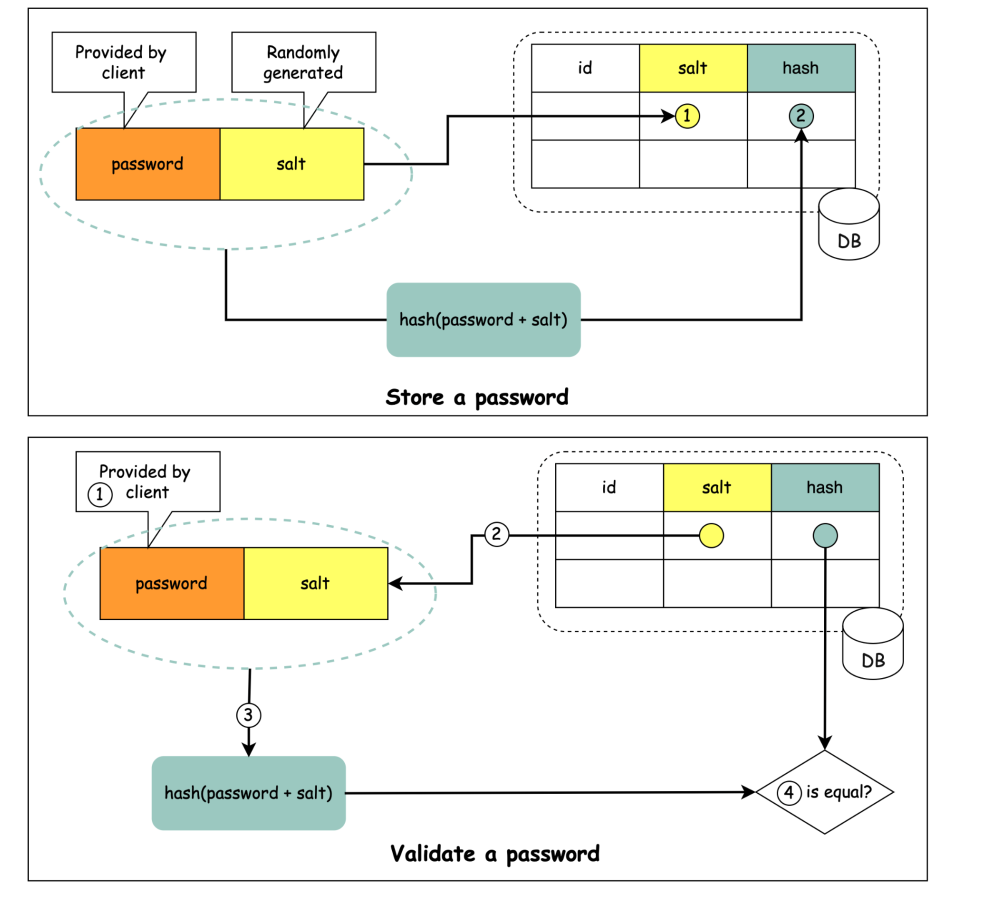
\includegraphics[width=0.5\linewidth]{images/StorePassword.png}
    \caption{Luu trữ mật khẩu trong ASP.NET Membership}
    \label{fig:StorePassword}
\end{figure}

Hình ảnh \ref{fig:StorePassword} minh họa quá trình lưu trữ và xác thực mật khẩu trong hệ thống. Đầu tiên, khi người dùng đăng ký tài khoản và cung cấp mật khẩu, một giá trị salt ngẫu nhiên được tạo ra để kết hợp với mật khẩu này. Salt là một chuỗi ngẫu nhiên được thêm vào mật khẩu trước khi thực hiện quá trình băm, giúp tăng cường bảo mật bằng cách ngăn chặn các tấn công dạng từ điển hoặc rainbow table. Sau đó, mật khẩu và salt được kết hợp và băm bằng hàm băm (SHA-1 trong trường hợp này). Kết quả băm cùng với salt và định danh người dùng (id) được lưu trữ vào cơ sở dữ liệu, đảm bảo rằng mỗi mật khẩu có một chuỗi băm duy nhất, ngay cả khi người dùng khác nhau sử dụng cùng một mật khẩu.

Quá trình xác thực mật khẩu diễn ra khi người dùng đăng nhập. Người dùng nhập mật khẩu và hệ thống sẽ truy xuất giá trị salt tương ứng từ cơ sở dữ liệu. Mật khẩu nhập vào được kết hợp với salt đã lấy và băm lại, giống như quá trình băm khi lưu trữ mật khẩu. Kết quả băm mới này sau đó được so sánh với chuỗi băm đã được lưu trữ trong cơ sở dữ liệu. Nếu hai giá trị băm trùng khớp, mật khẩu là chính xác và người dùng được xác thực; nếu không, quá trình xác thực thất bại.

Việc sử dụng salt và hàm băm để lưu trữ mật khẩu giúp tăng cường bảo mật cho hệ thống. Bằng cách kết hợp mật khẩu với một giá trị salt ngẫu nhiên trước khi băm, hệ thống bảo vệ mật khẩu khỏi các tấn công dạng từ điển hoặc rainbow table. Quá trình xác thực mật khẩu đảm bảo rằng mật khẩu nhập vào phải khớp với mật khẩu đã được băm và lưu trữ trong cơ sở dữ liệu, từ đó đảm bảo an toàn và tính toàn vẹn của hệ thống.

\begin{mdframed}[backgroundcolor=white, linecolor=black, roundcorner=5pt]
\begin{alltt}
CreateUser(string username, string password, string email, 
string securityQuestion, string securityAnswer, bool isApproved, 
object providerUserKey, out MembershipCreateStatus status)
\{
    string salt = GenerateSalt();
    string hashedPassword = HashPassword(password, Convert.FromBase64String(salt));
    Guid userId = Guid.NewGuid();

    using (NpgsqlConnection conn = new NpgsqlConnection(_connectionString))
    \{
        conn.Open();
        using (var transaction = conn.BeginTransaction())
        \{
            try
            \{                       
                using (NpgsqlCommand cmd = new NpgsqlCommand("SELECT 1 FROM aspnet_users 
                WHERE username = @username AND applicationname = @applicationname LIMIT 1"
                , conn))
                \{
                    cmd.Parameters.AddWithValue("username", username);
                    cmd.Parameters.AddWithValue("applicationname", "applicationname");

                    using (var reader = cmd.ExecuteReader())
                    \{
                        if (reader.HasRows)
                        \{
                            status = MembershipCreateStatus.DuplicateUserName;
                            return;
                        \}
                    \}
                \}

                using (NpgsqlCommand cmd = new NpgsqlCommand("INSERT INTO aspnet_users 
                (userid, username, applicationname) 
                VALUES (@userid, @username, @applicationname)", 
                conn))
                \{
                    cmd.Parameters.AddWithValue("userid", userId);
                    cmd.Parameters.AddWithValue("username", username);
                    cmd.Parameters.AddWithValue("applicationname", "applicationname");
                    cmd.ExecuteNonQuery();
                \}

                using (NpgsqlCommand cmd = new NpgsqlCommand("INSERT INTO aspnet_membership 
                (userid, password, passwordsalt, passwordformat, email
                , passwordquestion, passwordanswer, isapproved,
                islockedout, creationdate, lastlogindate,
                lastpasswordchangeddate) 
                VALUES (@userid, @password, @passwordsalt, @passwordformat,
                @email, @passwordquestion, @passwordanswer,
                @isapproved, @islockedout, @creationdate, @lastlogindate,
                @lastpasswordchangeddate)", conn))
                \{
                    cmd.Parameters.AddWithValue("userid", userId);
                    cmd.Parameters.AddWithValue("password", hashedPassword);
                    cmd.Parameters.AddWithValue("passwordsalt", salt);
                    cmd.Parameters.AddWithValue("passwordformat", 1);
                    cmd.Parameters.AddWithValue("email", email);
                    cmd.Parameters.AddWithValue("passwordquestion", securityQuestion);
                    cmd.Parameters.AddWithValue("passwordanswer", securityAnswer);
                    cmd.Parameters.AddWithValue("isapproved", isApproved ? 1 : 0);
                    cmd.Parameters.AddWithValue("islockedout", false ? 1 : 0);
                    cmd.Parameters.AddWithValue("creationdate", DateTime.UtcNow);
                    cmd.Parameters.AddWithValue("lastlogindate", DateTime.UtcNow);
                    cmd.Parameters.AddWithValue("lastpasswordchangeddate", DateTime.UtcNow);
                    cmd.ExecuteNonQuery();
                \}

                transaction.Commit();
                status = MembershipCreateStatus.Success;
            \}
            catch (Exception ex)
            \{
                transaction.Rollback();
                status = MembershipCreateStatus.ProviderError;
                throw ex;
            \}
        \}
    \}
\}

ValidateUser(string username, string password)
\{
    try
    \{
        using (NpgsqlConnection conn = new NpgsqlConnection(_connectionString))
        \{
            conn.Open();
            using (NpgsqlCommand cmd = new NpgsqlCommand("SELECT m.password, m.passwordsalt 
            FROM aspnet_membership m JOIN aspnet_users u ON m.userid = u.userid 
            WHERE u.username = @username AND u.applicationname = @applicationname", conn))
            \{
                cmd.Parameters.AddWithValue("username", username);
                cmd.Parameters.AddWithValue("applicationname", "applicationname");

                using (NpgsqlDataReader reader = cmd.ExecuteReader())
                \{
                    if (reader.Read())
                    \{
                        string storedPassword = reader.GetString(0);
                        string storedSalt = reader.GetString(1);
                        string hashedPassword = HashPassword(password
                        , Convert.FromBase64String(storedSalt));

                        return storedPassword == hashedPassword;
                    \}
                \}
            \}
        \}
    \}
    catch (Exception ex)
    \{
       throw new ApplicationException("An error occurred while validating user.", ex);
    \}

    return false;
\}

GenerateSalt()
\{
    byte[] saltBytes = new byte[16];
    using (var rng = new RNGCryptoServiceProvider())
    \{
        rng.GetBytes(saltBytes);
    \}
    return Convert.ToBase64String(saltBytes);
\}

HashPassword(string password, byte[] salt)
\{
    byte[] passwordBytes = Encoding.Unicode.GetBytes(password);
    byte[] saltedPasswordBytes = new byte[passwordBytes.Length + salt.Length];

    Buffer.BlockCopy(salt, 0, saltedPasswordBytes, 0, salt.Length);
    Buffer.BlockCopy(passwordBytes, 0, saltedPasswordBytes, salt.Length, passwordBytes.Length);

    using (SHA1 sha1 = SHA1.Create())
    \{
        byte[] hashBytes = sha1.ComputeHash(saltedPasswordBytes);
        return Convert.ToBase64String(hashBytes);
    \}
\}
\end{alltt}
\end{mdframed}

Trong đó:

CreateUser hàm này nhận các tham số: username, password, email, securityQuestion, securityAnswer, isApproved, providerUserKey, và status. Mục đích là tạo một người dùng mới trong hệ thống với thông tin được cung cấp, kiểm tra xem người dùng đã tồn tại hay chưa, và lưu trữ mật khẩu mã hóa cùng các thông tin liên quan vào cơ sở dữ liệu Greenplum. Cách thức hoạt động: Tạo một salt ngẫu nhiên, mã hóa mật khẩu bằng SHA1 với salt, tạo một Guid mới cho userId, kết nối với cơ sở dữ liệu Greenplum và thực hiện các truy vấn để kiểm tra và chèn thông tin người dùng vào các bảng aspnet\_users và aspnet\_membership.


ValidateUser hàm này nhận username và password làm tham số. Mục đích là xác thực người dùng bằng cách so sánh mật khẩu nhập vào với mật khẩu lưu trữ trong cơ sở dữ liệu. Cách thức hoạt động: Kết nối với cơ sở dữ liệu Greenplum, lấy mật khẩu và salt từ bảng aspnet\_membership, mã hóa mật khẩu nhập vào bằng salt, và so sánh mật khẩu đã mã hóa với mật khẩu lưu trữ.


GenerateSalt hàm này không nhận tham số. Mục đích là tạo một salt ngẫu nhiên để sử dụng trong việc mã hóa mật khẩu. Cách thức hoạt động: Sử dụng RNGCryptoServiceProvider để tạo một mảng byte ngẫu nhiên, sau đó chuyển đổi mảng byte này thành chuỗi Base64 để lưu trữ và sử dụng.


HashPassword hàm này nhận password và salt làm tham số. Mục đích là mã hóa mật khẩu bằng cách sử dụng salt để đảm bảo tính bảo mật cao hơn. Cách thức hoạt động: Chuyển đổi mật khẩu và salt thành mảng byte, kết hợp mảng byte của mật khẩu và salt, sử dụng hàm SHA1 để băm mảng byte kết hợp, và chuyển đổi kết quả băm thành chuỗi Base64 để lưu trữ.

Đoạn mã trên minh họa cách tạo và xác thực người dùng trong Greenplum với việc mã hóa mật khẩu tương tự như MSSQL. Bằng cách thực hiện các bước này có thể duy trì tính toàn vẹn và bảo mật của hệ thống trong suốt quá trình chuyển đổi. Việc sử dụng salt và hàm băm để lưu trữ mật khẩu giúp tăng cường bảo mật cho hệ thống. Quá trình xác thực mật khẩu đảm bảo rằng mật khẩu nhập vào phải khớp với mật khẩu đã được băm và lưu trữ trong cơ sở dữ liệu, từ đó đảm bảo an toàn và tính toàn vẹn của hệ thống.

\subsection{Kiểm thử}


\begin{figure}
    \centering
    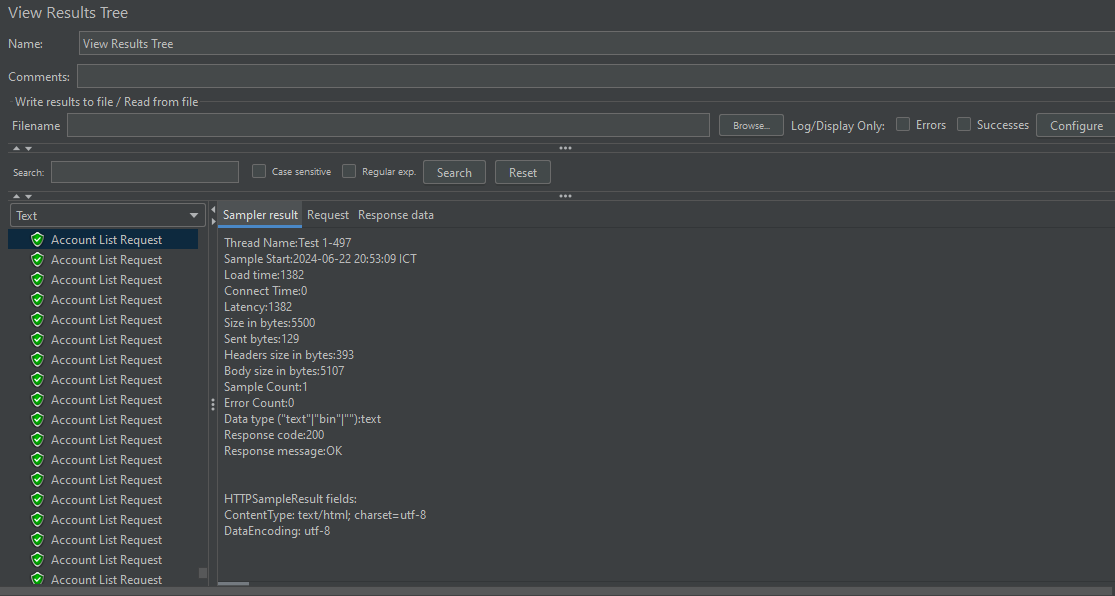
\includegraphics[width=0.8\linewidth]{images/vrt.png}
    \caption{View Results Tree trong JMeter}
    \label{fig:vrt}
\end{figure}

\begin{figure}
    \centering
    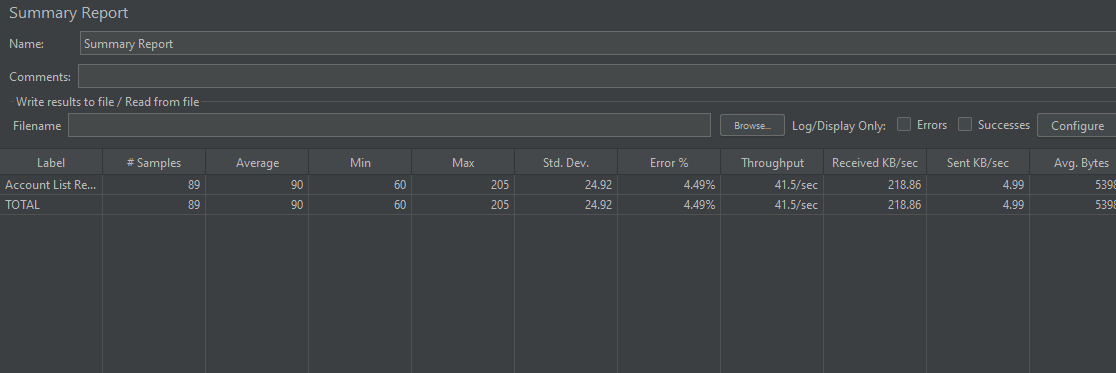
\includegraphics[width=0.8\linewidth]{images/sr.png}
     \caption{Summary Report trong JMeter}
    \label{fig:sr}
\end{figure}

\begin{figure}
    \centering
    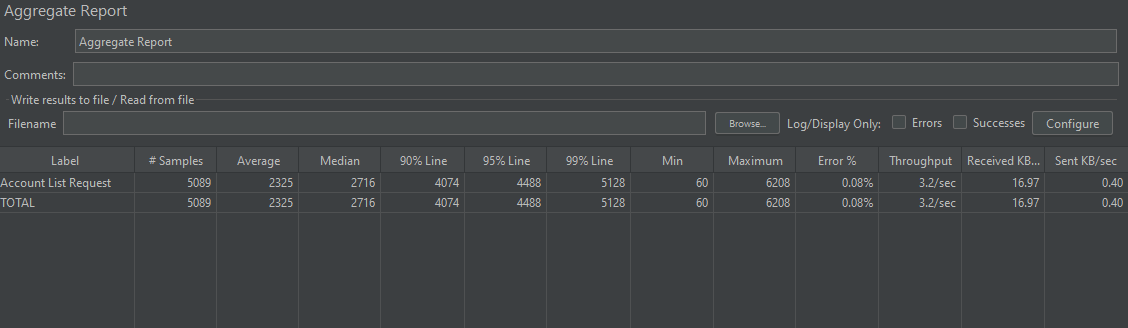
\includegraphics[width=0.8\linewidth]{images/ar.png}
    \caption{Aggregate Report trong JMeter}
    \label{fig:ar}
\end{figure}




Để thực hiện kiểm thử hiệu suất sử dụng Apache JMeter. Đầu tiên, truy cập trang chủ Apache JMeter\footnote{\url{https://jmeter.apache.org/download_jmeter.cgi}} và tải phiên bản mới nhất dưới dạng file ZIP hoặc TGZ. Sau khi giải nén file tải về vào một thư mục trên máy tính, cần cài đặt Java Development Kit (JDK) từ trang chủ Oracle JDK, chạy file cài đặt và thiết lập biến môi trường JAVA\_HOME trỏ tới thư mục cài đặt JDK, ví dụ: \verb|C:\Program Files\Java\jdk-11|. Chạy file jmeter.bat (trên Windows) hoặc jmeter (trên Unix/Linux) để khởi động giao diện người dùng của JMeter.


Trong JMeter, Thread Group là thành phần cốt lõi, nơi xác định số lượng người dùng ảo (threads) sẽ tương tác đồng thời với hệ thống. Để thêm Thread Group, chọn Add > Threads (Users) > Thread Group.

Listeners trong JMeter đóng vai trò quan trọng trong việc theo dõi, ghi nhận và trực quan hóa kết quả kiểm thử. Để thêm Listener vào Thread Group, chọn Add > Listener > Summary Report, Aggregate Report, View Results Tree như minh họa trong hình \ref{fig:testjmeter}.

Việc chuyển đổi dữ liệu từ MSSQL sang Greenplum đòi hỏi một bước kiểm định hiệu suất quan trọng để đảm bảo hệ thống mới vận hành mượt mà và đáp ứng mọi yêu cầu hiệu suất. Apache JMeter để tiến hành các bài kiểm thử toàn diện, đánh giá khả năng xử lý tải cao, độ tin cậy, và khả năng mở rộng của hệ thống.

JMeter đóng vai trò trung tâm trong quá trình kiểm thử, với Thread Group là thành phần cốt lõi. Thread Group cho phép xác định số lượng người dùng ảo (threads) tương tác đồng thời với Greenplum, mô phỏng các mức tải khác nhau, từ thấp đến cao, để đánh giá khả năng đáp ứng của hệ thống trong điều kiện thực tế.

Samplers trong JMeter, như HTTP Request Sampler, được sử dụng để gửi các yêu cầu (GET, POST) đến các điểm cuối cụ thể của Greenplum, mô phỏng hành vi người dùng thực. JMeter sẽ ghi lại kết quả trả về từ Greenplum để phân tích và đánh giá.

Listeners trong JMeter đóng vai trò quan trọng trong việc giám sát, ghi nhận và trực quan hóa kết quả kiểm thử. View Results Tree như hình \ref{fig:vrt} cung cấp chi tiết từng yêu cầu và phản hồi, giúp xác định các vấn đề cụ thể. Summary Report như hình \ref{fig:sr} tổng hợp thông tin hiệu suất hệ thống, bao gồm thời gian phản hồi trung bình, độ lệch chuẩn, và tỷ lệ yêu cầu thành công/thất bại. Aggregate Report như hình \ref{fig:ar} cung cấp dạng bảng tổng hợp các số liệu thống kê quan trọng như trung bình, trung vị, min, max, và phân vị 90\%, 95\%, 99\% của thời gian phản hồi. Các listener này cung cấp cái nhìn toàn diện về hoạt động của Greenplum dưới áp lực tải, từ đó đưa ra các điều chỉnh và tối ưu hóa cần thiết.

\subsection{Phân tích so sánh}






\section{Kết luận}
Bổ sung sau

\section{Phụ lục}
\appendix

\section{Các bước triển khai}




\subsection{Cài đặt Greenplum}

Trước khi cài đặt Greenplum, cần phải cài đặt các gói phụ trợ cần thiết để đảm bảo môi trường hoạt động tốt. Thực hiện lệnh sau để cài đặt các gói này với đúng phiên bản yêu cầu:
\begin{verbatim}
sudo yum install -y \
    apr-1.6.3-12.el8 \
    apr-util-1.6.1-9.el8 \
    bzip2-1.0.6-26.el8 \
    krb5-devel-1.18.2-25.el8 \
    libcgroup-tools-0.41-19.el8 \
    net-tools-2.0-0.52.20160912git.el8 \
    perl-4:5.26.3-422.el8 \
    zip-3.0-23.el8 \
    nano-2.9.8-1.el8.x86_64 \
    wget-1.19.5-11.el8
\end{verbatim}

Dùng wget để tải gói Greenplum từ trang phát hành chính thức:

\begin{verbatim}
wget https://github.com/greenplum-db/gpdb/releases/download/6.25.1/open-source-greenplum-db-6.25.1-rhel8-x86_64.rpm
\end{verbatim}

Sử dụng lệnh sau để cài đặt gói Greenplum đã tải:

\begin{verbatim}
sudo rpm -ivh open-source-greenplum-db-6.25.1-rhel8-x86_64.rpm
\end{verbatim}

Tạo file hostfile\_gpinitsystem chứa các địa chỉ IP của các segment và coordinator:

\begin{verbatim}
nano /home/gpadmin/hostfile_gpinitsystem
\end{verbatim}

Sao chép file cấu hình và chỉnh sửa:

\begin{verbatim}
source /usr/local/greenplum-db-6.25.1/greenplum_path.sh
cp $GPHOME/docs/cli_help/gpconfigs/gpinitsystem_config .
nano gpinitsystem_config
\end{verbatim}

Chỉnh sửa file gpinitsystem\_config với các thông số cần thiết:

\begin{verbatim}
ARRAY_NAME="Greenplum Data Platform"
SEG_PREFIX=gpseg
PORT_BASE=6000
declare -a DATA_DIRECTORY=(/home/gpadmin/data1/primary /home/gpadmin/data1/primary /home/gpadmin/data)
MASTER_HOSTNAME=master
MASTER_DIRECTORY=/home/gpadmin/data/master
MASTER_PORT=5432
TRUSTED_SHELL=ssh
CHECK_POINT_SEGMENTS=8
ENCODING=UNICODE
DATABASE_NAME=Data1
MACHINE_LIST_FILE=/home/gpadmin/hostfile_gpinitsystem
\end{verbatim}

Khởi tạo hệ thống Greenplum

\begin{verbatim}
gpinitsystem -c gpinitsystem_config
\end{verbatim}

Sao chép file hostfile\_gpinitsystem

\begin{verbatim}
cp $GPHOME/docs/cli_help/gpconfigs/hostfile_gpinitsystem .
\end{verbatim}

Thiết lập SSH key để cho phép đăng nhập không cần mật khẩu:

\begin{verbatim}
gpssh-exkeys -f hostfile_gpinitsystem
\end{verbatim}

Trong đó file hostfile\_gpinitsystem chứa IP của các segment.

Thêm đường dẫn của MASTER\_DATA\_DIRECTORY vào /etc/environment

\begin{verbatim}
nano /etc/environment
MASTER_DATA_DIRECTORY="/home/gpadmin/data/master/gpseg-1"
\end{verbatim}

Khởi động hệ thống Greenplum:

\begin{verbatim}
gpstart -a
\end{verbatim}

Các bước trên đã hướng dẫn chi tiết cách chuẩn bị, cài đặt và cấu hình hệ thống Greenplum trên CentOS. Quy trình này bao gồm việc cài đặt các gói cần thiết, tải và cài đặt Greenplum, thiết lập passwordless SSH cho các segment, cấu hình và khởi tạo hệ thống Greenplum, cũng như thêm đường dẫn của MASTER\_DATA\_DIRECTORY và khởi động hệ thống Greenplum.



\subsection{Tích hợp provider sử dụng cho Greenplum}

Để tích hợp ASP.NET Membership với cơ sở dữ liệu Greenplum cần sử dụng provider của Devart là dotConnect for PostgreSQL. Quá trình này bao gồm việc tạo schema cần thiết trên Greenplum và cấu hình các provider trong file Web.config.

Đầu tiên cần truy cập vào trang chủ của Devart và tải schema mẫu dành cho ASP.NET Membership. Sau khi tải xuống, hãy tạo schema này trên cơ sở dữ liệu Greenplum.

Đầu tiên cần kết nối với Greenplum trong file Web.config.


\begin{mdframed}[backgroundcolor=white, linecolor=black, roundcorner=5pt]
\begin{alltt}
<add name="PgSqlServices" 
     connectionString="Server=IP_server;
                       Port=Port_Server;
                       Database=Name_Database;
                       User Id=IP_server;
                       Password=Password_server;"/>
</connectionStrings>
\end{alltt}
\end{mdframed}

Dưới đây là các cấu hình cần thiết trong file Web.config để sử dụng ASP.NET Membership, Roles, và Profile với Greenplum thông qua provider của Devart.

Cấu hình ASP.NET Membership
\begin{mdframed}[backgroundcolor=white, linecolor=black, roundcorner=5pt]
\begin{alltt}
<membership defaultProvider="AspNetPgSqlMembershipProvider"
            userIsOnlineTimeWindow="15">
  <providers>
    <add
      name="AspNetPgSqlMembershipProvider"
      type="Devart.Data.PostgreSql.Web.Providers.PgSqlMembershipProvider,
            Devart.Data.PostgreSql.Web, Version=8.3.20, Culture=neutral,
            PublicKeyToken=09af7300eec23701"
      connectionStringName="PgSqlServices"
      enablePasswordRetrieval="false"
      enablePasswordReset="true"
      requiresQuestionAndAnswer="true"
      requiresUniqueEmail="false"
      passwordFormat="Hashed"
      maxInvalidPasswordAttempts="5"
      passwordAttemptWindow="10" />
  </providers>
</membership>
\end{alltt}
\end{mdframed}

Cấu hình ASP.NET Role
\begin{mdframed}[backgroundcolor=white, linecolor=black, roundcorner=5pt]
\begin{alltt}
<roleManager defaultProvider="AspNetPgSqlRoleProvider"
             enabled="true"
             cacheRolesInCookie="true"
             cookieName=".ASPROLES"
             cookieTimeout="30"
             cookiePath="/"
             cookieProtection="All">
  <providers>
    <add
      name="AspNetPgSqlRoleProvider"
      type="Devart.Data.PostgreSql.Web.Providers.PgSqlRoleProvider,
            Devart.Data.PostgreSql.Web, Version=8.3.20, Culture=neutral,
            PublicKeyToken=09af7300eec23701"
      connectionStringName="PgSqlServices" />
  </providers>
</roleManager>
\end{alltt}
\end{mdframed}

Cấu hình ASP.NET Profile 
\begin{mdframed}[backgroundcolor=white, linecolor=black, roundcorner=5pt]
\begin{alltt}
<profile defaultProvider="AspNetPgSqlProfileProvider">
  <providers>
    <add
      name="AspNetPgSqlProfileProvider"
      type="Devart.Data.PostgreSql.Web.Providers.PgSqlProfileProvider,
            Devart.Data.PostgreSql.Web, Version=8.3.20, Culture=neutral,
            PublicKeyToken=09af7300eec23701"
      connectionStringName="PgSqlServices" />
  </providers>
  <properties>
    <add name="FirstName" />
    <add name="LastName" />
    <add name="DateOfBirth" type="System.DateTime"/>
  </properties>
</profile>
\end{alltt}
\end{mdframed}

Việc sử dụng dotConnect for PostgreSQL của Devart cho phép dễ dàng tích hợp ASP.NET Membership với cơ sở dữ liệu Greenplum. Quá trình này bao gồm việc tạo schema cần thiết và cấu hình các provider trong file Web.config.


\subsection{Dữ liệu}

\subsubsection{Chuẩn bị dữ liệu}

Dữ liệu này bao gồm thông tin về người dùng, quyền hạn, hồ sơ cá nhân và các giao dịch liên quan. Thông tin người dùng bao gồm: UserID, UserName, Email, Password, IsApproved, IsLockedOut, LastLoginDate, CreationDate. Quyền hạn bao gồm: RoleID, RoleName. Hồ sơ cá nhân bao gồm: FirstName, LastName, DateOfBirth, SecurityQuestion, SecurityAnswer.

Mã nguồn chuẩn bị dữ liệu kiểm thử:

\begin{mdframed}[backgroundcolor=white, linecolor=black, roundcorner=5pt]
\begin{alltt}
SeedUsers()
\{
    var random = new Random();
    int attempt = 5;
    for (int i = 0; i < 2000000; i++)
    \{
        bool isLocked = random.Next(2) == 1;
        var userName = $"member{i}";
        var password = $"Password123!";
        var email = $"user{i}@example.com";
        MembershipCreateStatus createStatus;
        MembershipUser newUser = Membership.CreateUser(
            userName, password, email,
            "What is your favorite color?", "Blue",
            isApproved: true, null, out createStatus);

        if (createStatus == MembershipCreateStatus.Success)
        \{
            if (isLocked)
            \{
                SimulateFailedLogins(userName, attempt);
            \}

            AssignUserToRandomRole(userName);

            try
            \{
                SaveUserProfile(userName, $"FirstName{i}", $"LastName{i}");
            \}
            catch (Exception profileEx)
            \{
                Console.WriteLine($"Error saving profile for user {userName}: {profileEx}");
            \}
        \}
        else
        \{
            Console.WriteLine(\$"Error creating user {userName}: {createStatus}");
        \}
    \}
\}

SimulateFailedLogins(string userName, int attempts)
\{
    for (int attempt = 0; attempt < attempts; attempt++)
    \{
        Membership.ValidateUser(userName, "wrongPassword");
    \}
\}

AssignUserToRandomRole(string userName)
\{
    var random = new Random();
    string[] roles = \{ "Admin", "User" \};
    string role = roles[random.Next(roles.Length)];
    Roles.AddUserToRole(userName, role);
\}

SaveUserProfile(string userName, string firstName, string lastName)
\{
    dynamic profile = ProfileBase.Create(userName, true);
    profile.SetPropertyValue("FirstName", firstName);
    profile.SetPropertyValue("LastName", lastName);
    profile.SetPropertyValue("DateOfBirth", new DateTime(1990, 1, 1).AddDays(new Random().Next(365)));
    profile.Save();
\}
\end{alltt}
\end{mdframed}

Trong đó:

SeedUsers: Hàm chính để tạo 2 triệu người dùng. Với mỗi người dùng, nó sẽ tạo thông tin cơ bản như userName, password, và email. Sau đó, gọi hàm Membership.CreateUser để tạo người dùng.
SimulateFailedLogins: Giả lập các lần đăng nhập thất bại để khóa tài khoản người dùng.
AssignUserToRandomRole: Gán người dùng vào một quyền hạn ngẫu nhiên.
SaveUserProfile: Lưu hồ sơ cá nhân của người dùng, bao gồm FirstName, LastName, và DateOfBirth.

\subsubsection{Chuyển dữ liệu}

Trong quá trình chuyển đổi dữ liệu từ MSSQL sang Greenplum, Pentaho Data Integration (PDI) được sử dụng để thực hiện các thao tác ETL (Extract, Transform, Load). Dưới đây là các bước chi tiết cho quá trình này.

Đầu tiên cần kết nối MSSQL và greenplum trong phần Database connection PDI như hình \ref{fig:ConMSSQL}, \ref{fig:ConGreenplum}.


\begin{figure}
    \centering
    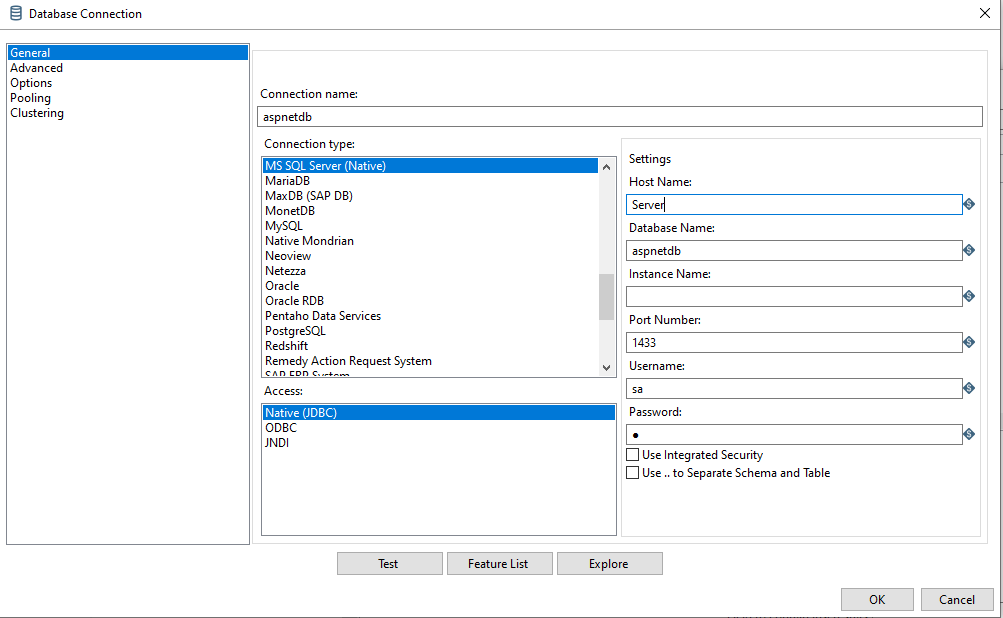
\includegraphics[width=0.8\linewidth]{images/ConMSSQL.png}
    \caption{Kết nối PDI với MSSQL}
    \label{fig:ConMSSQL}
\end{figure}


\begin{figure}
    \centering
    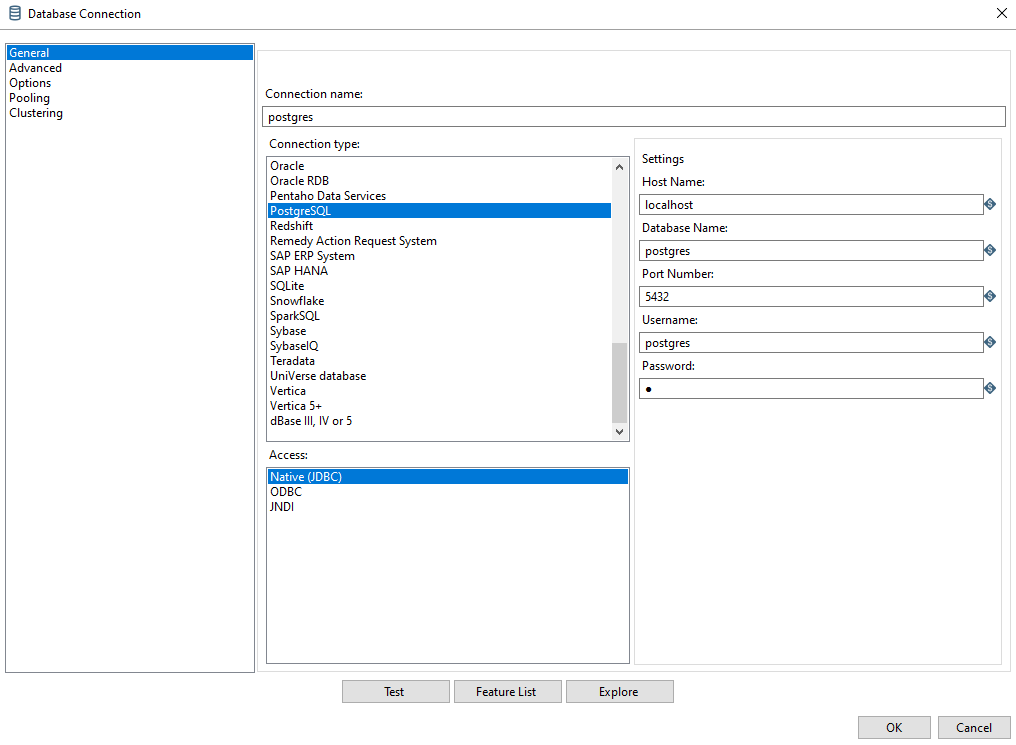
\includegraphics[width=0.8\linewidth]{images/ConGreenplum.png}
    \caption{Kết nối PDI với Greenplum}
    \label{fig:ConGreenplum}
\end{figure}

\begin{figure}
    \centering
    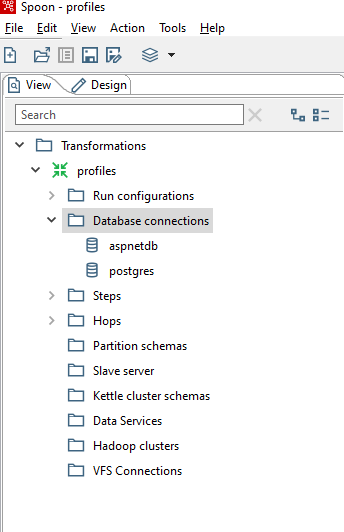
\includegraphics[width=0.8\linewidth]{images/ComMSGL.png}
    \caption{Kết nói thành công MSSQL và Greenplum}
    \label{fig:ComMSGL}
\end{figure}


Hình \ref{fig:ComMSGL} khi kết nối thành công MSSQL và Greenplum 


Quá trình chuyển dữ liệu bằng Pentaho được thực hiện qua các bước chính sau đây:

Khởi đầu quá trình bằng việc thiết lập một bản thiết kế tổng quát cho quy trình ETL trong Pentaho. Mục tiêu là tạo ra một luồng công việc tự động, bao gồm các bước từ truy vấn dữ liệu từ nguồn MSSQL, xử lý và chuyển đổi dữ liệu, đến việc tải dữ liệu vào đích Greenplum.

Sử dụng công cụ Table Input của Pentaho để truy vấn và trích xuất dữ liệu từ cơ sở dữ liệu MSSQL. Các truy vấn SQL được sử dụng để lấy dữ liệu từ các bảng như roles, users, usersinroles, profiles, và membership.

Hình \ref{fig:roles} sử dụng Table Input để lấy thông tin role trong bảng aspnet\_Roles

\begin{figure}
    \centering
    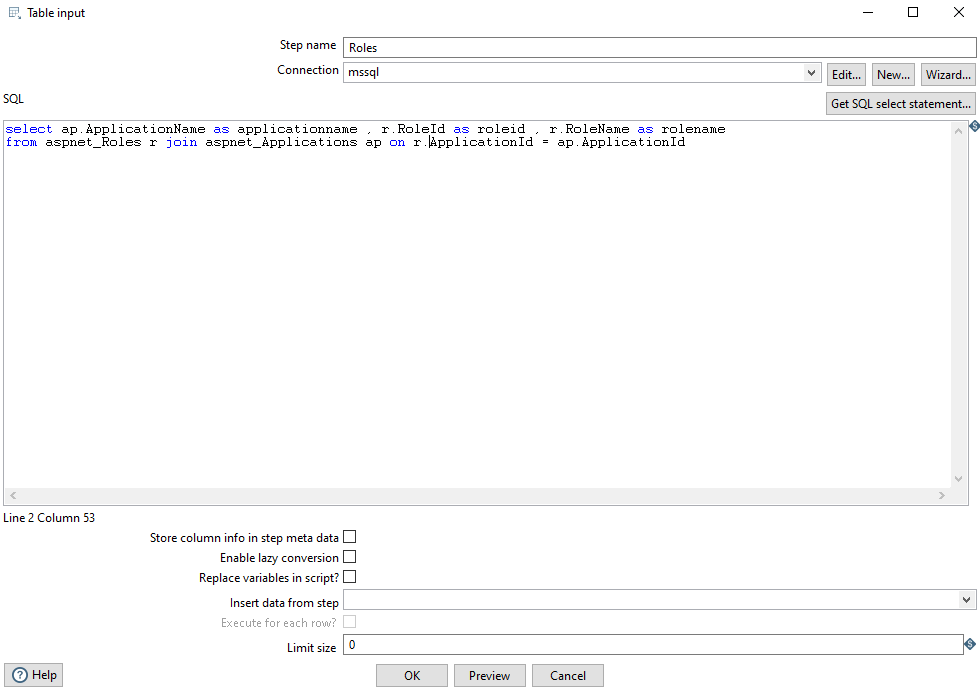
\includegraphics[width=0.8\linewidth]{images/roles.png}
    \caption{Table Input của aspnet\_Roles của MSSQL}
    \label{fig:roles}
\end{figure}

Hình \ref{fig:usersl} sử dụng Table Input để lấy thông tin users trong bảng aspnet\_Users

\begin{figure}
    \centering
    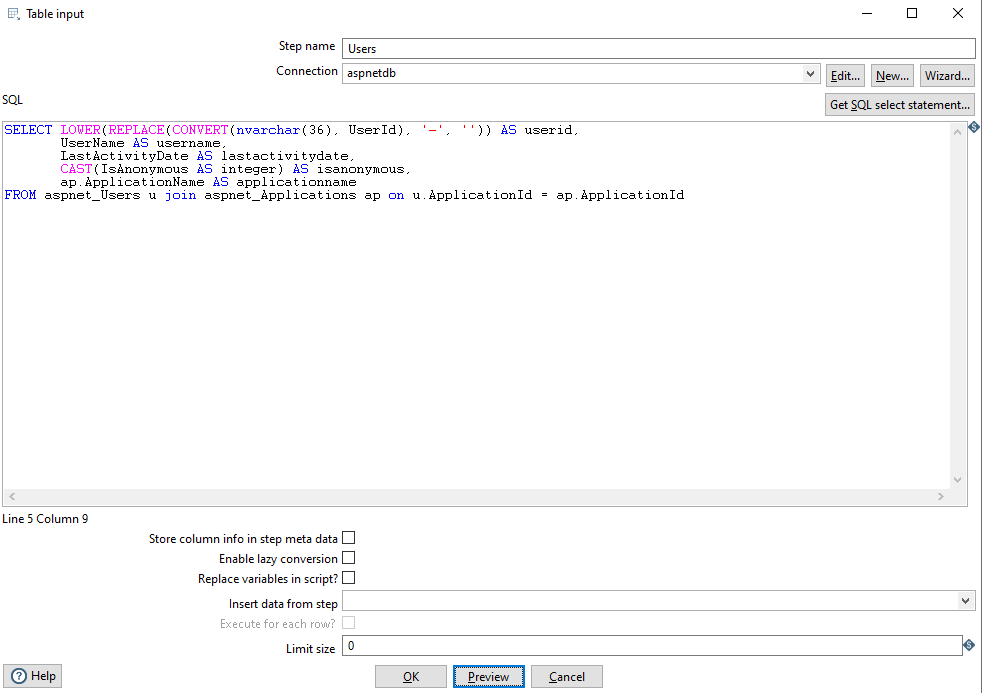
\includegraphics[width=0.5\linewidth]{images/users.png}
    \caption{Table Input của aspnet\_Users của MSSQL}
    \label{fig:usersl}
\end{figure}

Hình \ref{fig:UsersInRoles} sử dụng Table Input để lấy thông tin role trong bảng aspnet\_UsersInRoles

\begin{figure}
    \centering
    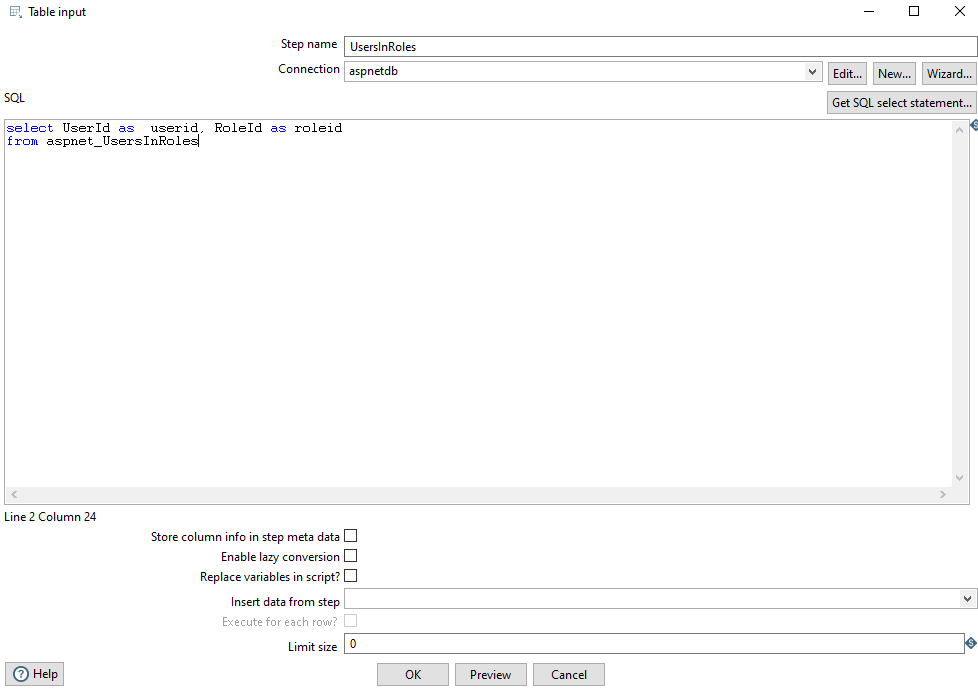
\includegraphics[width=0.5\linewidth]{images/UsersInRoles.png}
    \caption{Table Input của aspnet\_UsersInRoles của MSSQL}
    \label{fig:UsersInRoles}
\end{figure}

Hình \ref{fig:Membership} sử dụng Table Input để lấy thông tin Membership trong bảng aspnet\_Membership

\begin{figure}
    \centering
    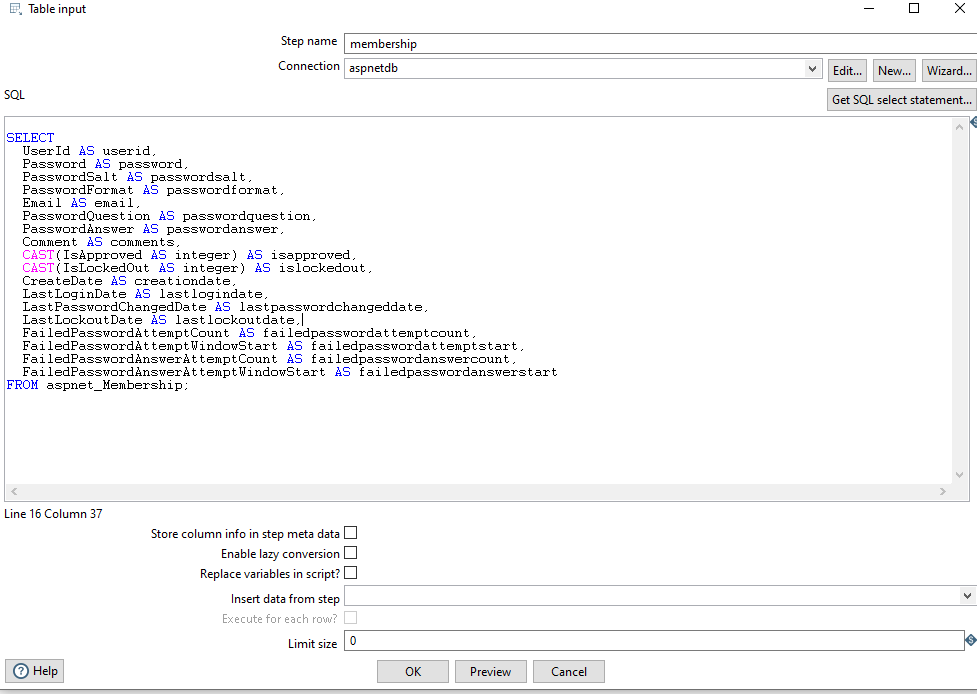
\includegraphics[width=0.5\linewidth]{images/Membership.png}
    \caption{Table Input của aspnet\_Membership của MSSQL}
    \label{fig:Membership}
\end{figure}

Hình \ref{fig:Profile} sử dụng Table Input để lấy thông tin profile trong bảng aspnet\_Profile

\begin{figure}
    \centering
    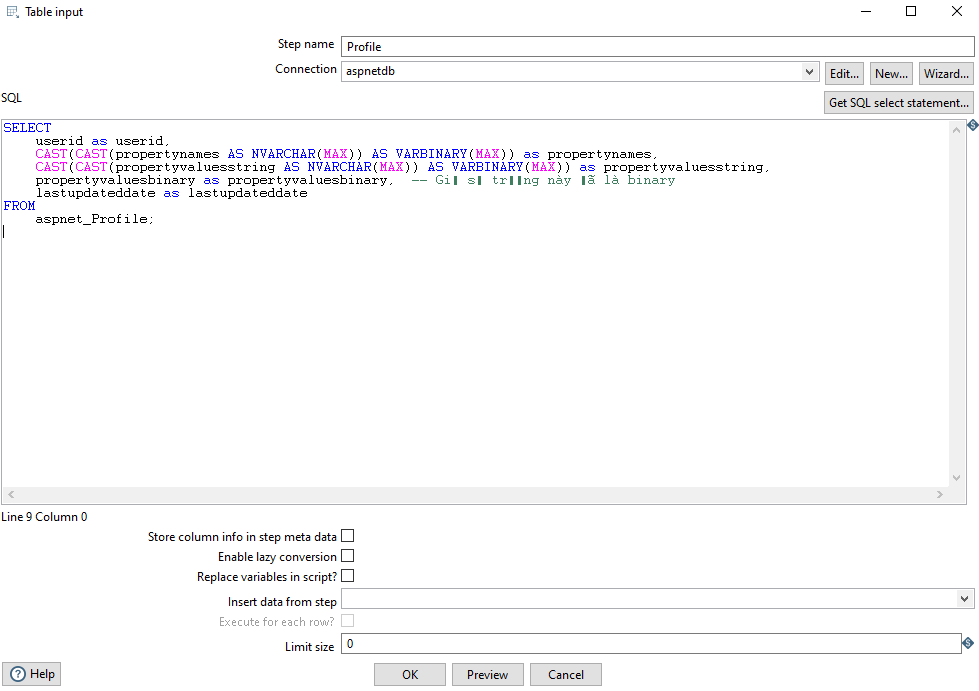
\includegraphics[width=0.5\linewidth]{images/Profile.png}
   \caption{Table Input của aspnet\_Profile của MSSQL}
    \label{fig:Profile}
\end{figure}



Sử dụng công cụ Execute SQL script của Pentaho để nhận dữ liệu từ các bảng như aspnet\_roles, aspnet\_users, aspnet\_usersinroles, aspnet\_profiles, và aspnet\_membership.

Hình \ref{fig:groles} sử dụng Execute SQL script để lấy thông tin roles trong bảng aspnet\_roles của Greenplum


\begin{figure}
    \centering
    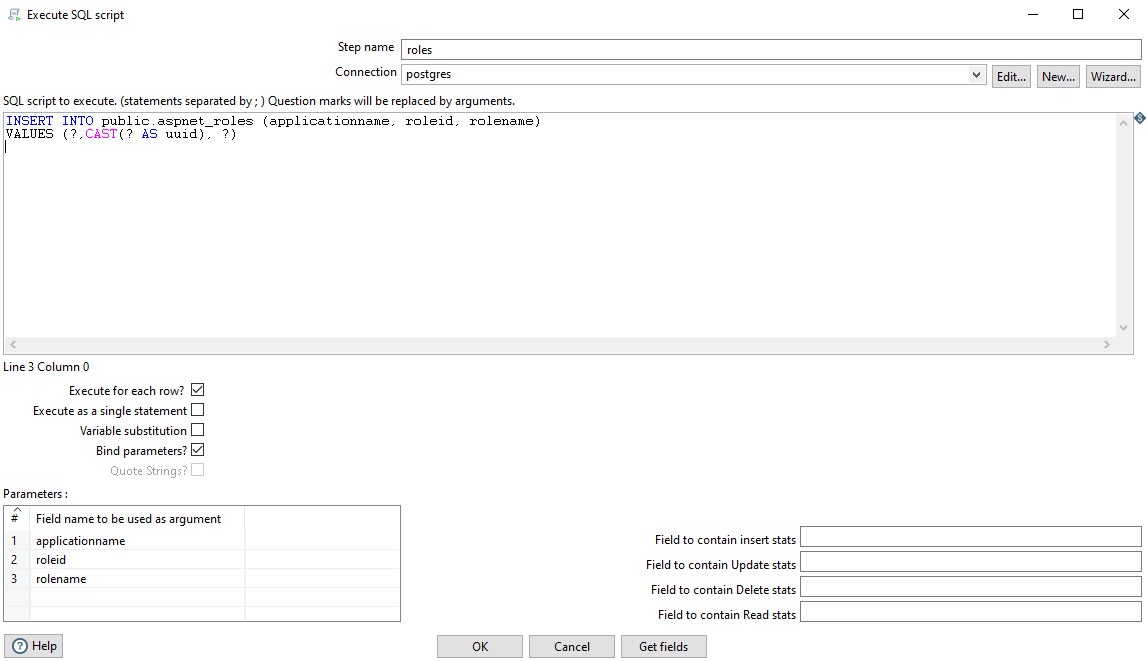
\includegraphics[width=0.5\linewidth]{images/groles.png}
     \caption{Execute SQL script aspnet\_roles của Greenplum}
    \label{fig:groles}
\end{figure}

Hình \ref{fig:gusers} sử dụng Execute SQL script để lấy thông tin users trong bảng aspnet\_users của Greenplum


\begin{figure}
    \centering
    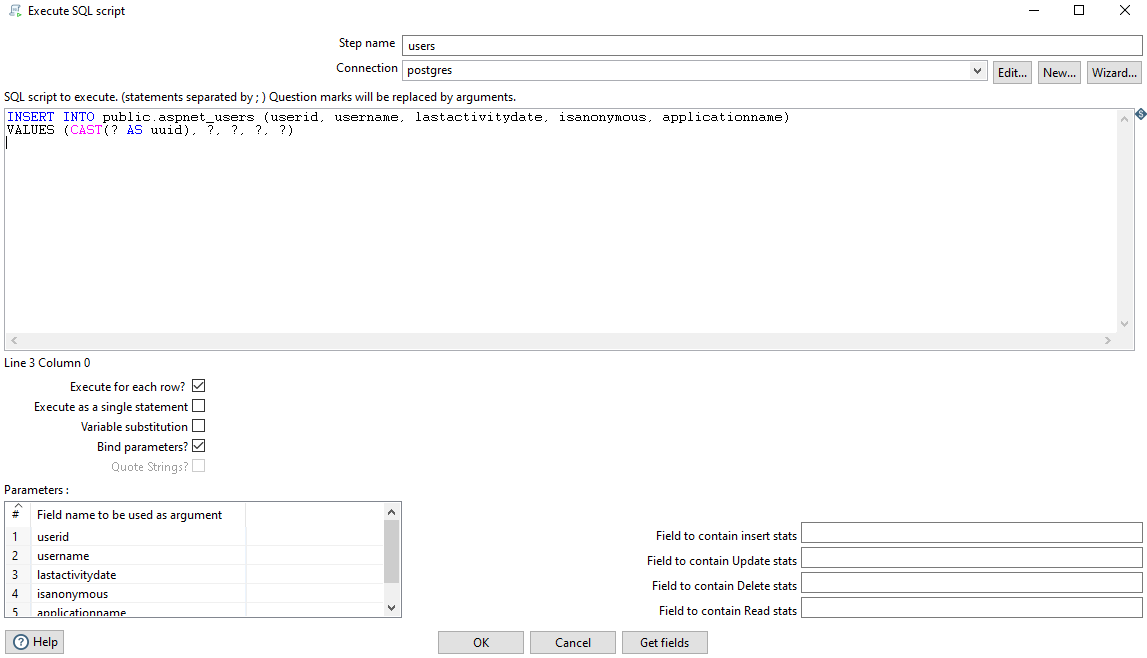
\includegraphics[width=0.5\linewidth]{gusers.png}
     \caption{Execute SQL script aspnet\_users của Greenplum}
    \label{fig:gusers}
\end{figure}

Hình \ref{fig:gusersinroles} sử dụng Execute SQL script để lấy thông tin usersinroles trong bảng aspnet\_usersinroles của Greenplum


\begin{figure}
    \centering
    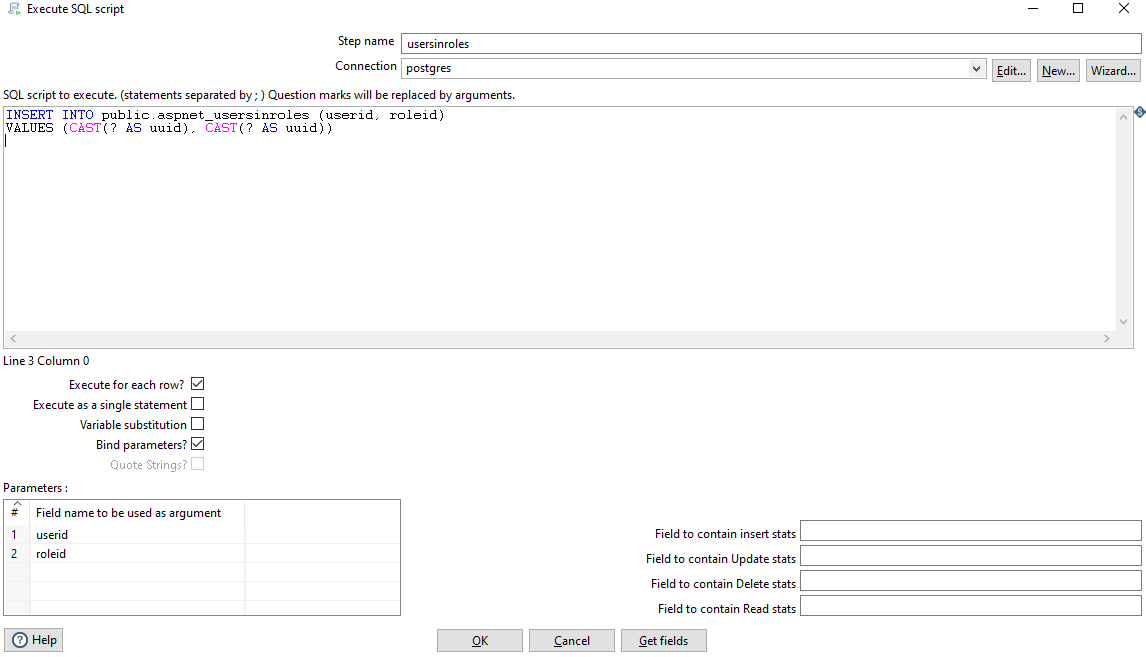
\includegraphics[width=0.5\linewidth]{images/gusersinroles.png}
    \caption{Execute SQL script aspnet\_usersinroles của Greenplum}
    \label{fig:gusersinroles}
\end{figure}

Hình \ref{fig:gmembership} sử dụng Execute SQL script để lấy thông tin membership trong bảng aspnet\_membership của Greenplum


\begin{figure}
    \centering
    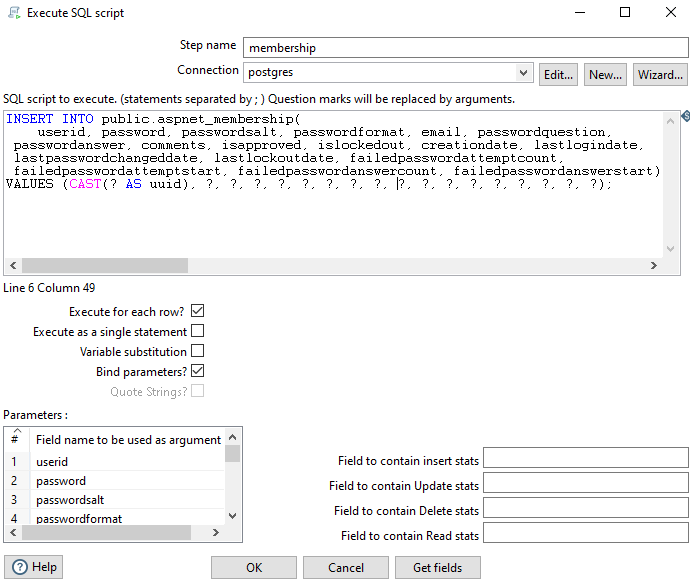
\includegraphics[width=0.5\linewidth]{images/gmembership.png}
     \caption{Execute SQL script aspnet\_membership của Greenplum}
    \label{fig:gmembership}
\end{figure}

Hình \ref{fig:gprofiles} sử dụng Execute SQL script để lấy thông tin roles trong bảng aspnet\_roles của Greenplum


\begin{figure}
    \centering
    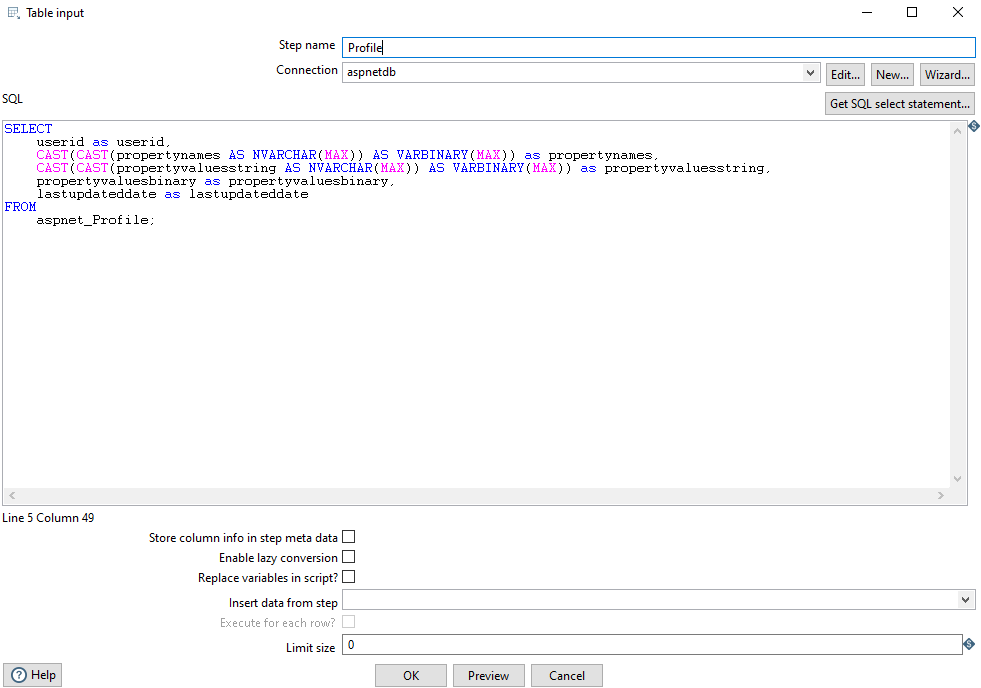
\includegraphics[width=0.5\linewidth]{images/gprofiles.png}
    \caption{Execute SQL script aspnet\_profiles của Greenplum}
    \label{fig:gprofiles}
\end{figure}


Cuối cùng như hình \ref{fig:job} sử dụng Job để sử dụng các transformation để hoàn chỉnh ETL của PDI


\begin{figure}
    \centering
    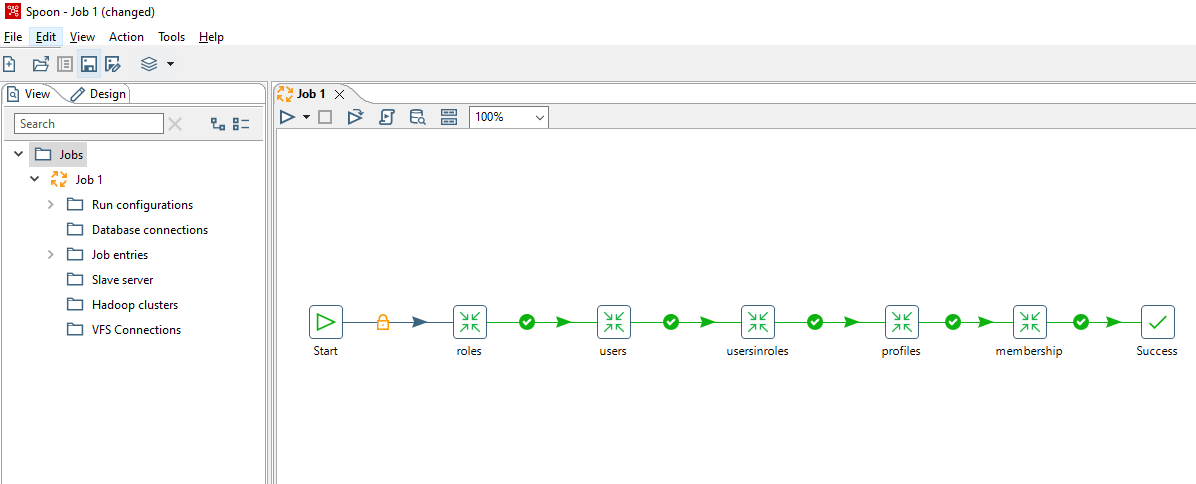
\includegraphics[width=0.5\linewidth]{images/job.png}
    \caption{Job ETL}
    \label{fig:job}
\end{figure}



\subsection{Giao diện}



Như hình \ref{fig:day} hiển thị thống kê người dùng trong hệ thống ASP.NET Membership cung cấp cái nhìn tổng quan về số lượng người dùng và tình trạng tài khoản. Thẻ "Members" màu xanh hiển thị tổng số lượng người dùng và thẻ "Blocked" màu đỏ hiển thị số lượng người dùng bị khóa , giúp quản trị viên dễ dàng theo dõi và quản lý. Biểu đồ dạng đường hiển thị số lượng người dùng đăng nhập hàng ngày trong tháng 6/2024. Bộ lọc thời gian (Day, Week, Month, Year) giúp linh hoạt trong việc phân tích dữ liệu. Giao diện này hỗ trợ quản lý hiệu quả, phân tích xu hướng và phát hiện, xử lý các vấn đề liên quan đến tài khoản người dùng, đảm bảo hệ thống hoạt động ổn định và hiệu quả.




Hình ảnh \ref{fig:list} thể hiện giao diện quản lý người dùng trong hệ thống ASP.NET Membership. Giao diện lọc người dùng theo các tiêu chí khác nhau như đăng nhập gần đây, bị khóa, và không đăng nhập trong tháng qua. Dữ liệu hiển thị trên bảng bao gồm thông tin số thứ tự, tên đăng nhập, họ, tên, email và lần đăng nhập cuối cùng của người dùng.

\subsection{Kiểm thử}

Để cài đặt Apache JMeter truy cập trang chủ Apache JMeter\footnote{\url{https://jmeter.apache.org/download_jmeter.cgi}} và tải phiên bản mới nhất dưới dạng file ZIP hoặc TGZ. Sau khi giải nén file đã tải về vào một thư mục trên máy tính, cần cài đặt Java Development Kit (JDK) bằng cách tải từ trang chủ Oracle JDK\footnote{\url{https://www.oracle.com/java/technologies/downloads/}}, chạy file cài đặt và thiết lập biến môi trường JAVA\_HOME trỏ tới thư mục cài đặt JDK. ví dụ: \begin{verbatim}C:\Program Files\Java\jdk-11\end{verbatim}

Chạy file jmeter.bat (trên Windows) hoặc jmeter (trên Unix/Linux) để khởi động giao diện người dùng của JMeter.

Trong JMeter, Thread Group là thành phần cốt lõi, nơi xác định số lượng người dùng ảo (threads) sẽ tương tác đồng thời với hệ thống. Để thêm Thread Group, chọn Add > Threads (Users) > Thread Group.

Listeners trong JMeter đóng vai trò quan trọng trong việc theo dõi, ghi nhận và trực quan hóa kết quả kiểm thử. Để thêm Listener vào Thread Group, chọn Add > Listener > Summary Report, Aggregate Report, View Results Tree như hình \ref{fig:testjmeter}.


\begin{figure}
    \centering
    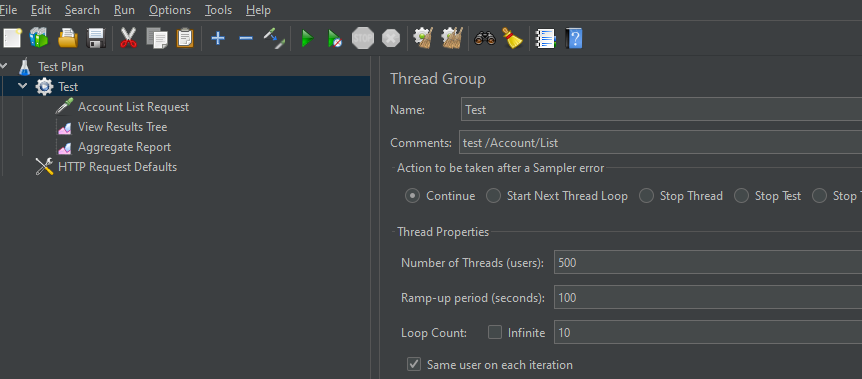
\includegraphics[width=0.5\linewidth]{images/testjmeter.png}
    \caption{Thông số test trong JMeter}
    \label{fig:testjmeter}
\end{figure}

\begin{figure}
    \centering
    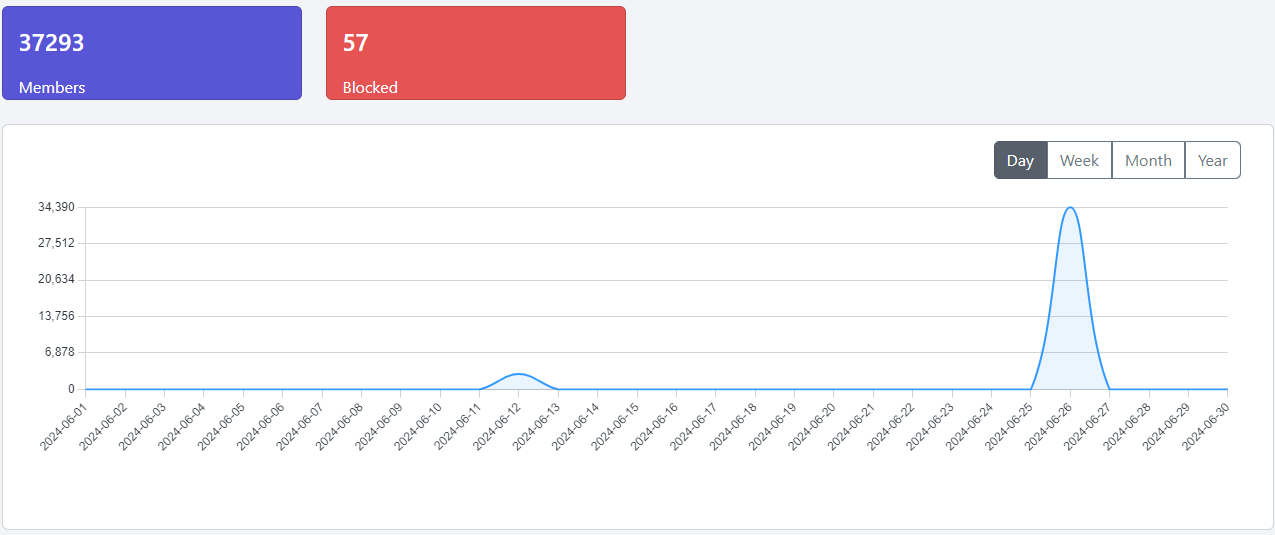
\includegraphics[width=0.5\linewidth]{images/day.png}
    \caption{Giao diện hiển thị thống kê người dùng trong hệ thống ASP.NET Membership}
    \label{fig:day}
\end{figure}


\begin{figure}
    \centering
    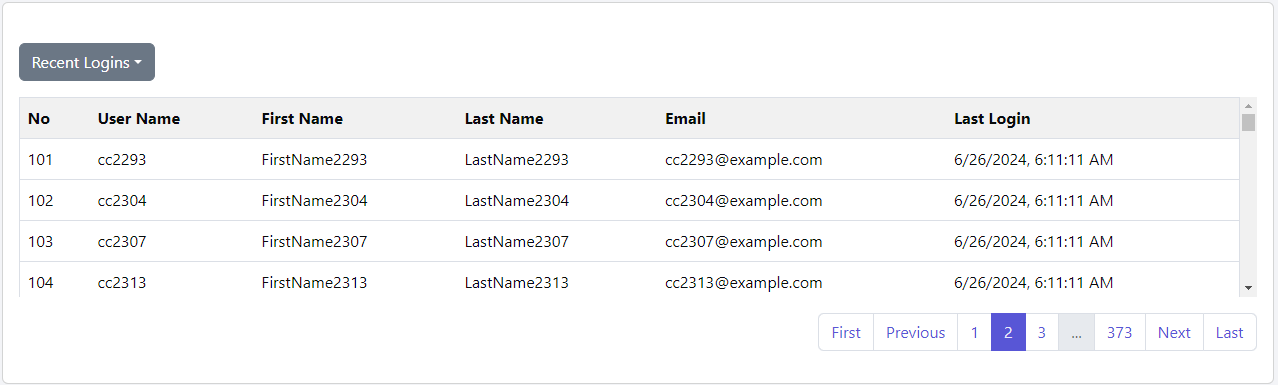
\includegraphics[width=0.8\linewidth]{images/list.png}
    \caption{Giao diện hiển thị danh sách người dùng trong hệ thống ASP.NET Membership}
    \label{fig:list}
\end{figure}
    
    
   
    \pagebreak 
    %TÀI LIỆU TRÍCH DẪN
    %Đây là ví dụ
    \bibliographystyle{ieeetr}
    \bibliography{References/references}
    \nocite{*}

    

\end{document}